\documentclass[11pt]{article}
\usepackage[utf8]{inputenc}
\usepackage{graphicx}
\usepackage{amsmath}
\usepackage{mathrsfs}


%%%%%%%%%% To get three levels of sub sections
\usepackage{titlesec}
\setcounter{secnumdepth}{4}
\titleformat{\paragraph}
{\normalfont\normalsize\bfseries}{\theparagraph}{1em}{}
\titlespacing*{\paragraph}
{0pt}{3.25ex plus 1ex minus .2ex}{1.5ex plus .2ex}


%%%%%%%%%%Positioning of graphics figures
\usepackage{float}
\usepackage{subcaption}
\usepackage{amssymb,amsthm,amsmath}   
\graphicspath{{0_images/}}
\usepackage{geometry}
\usepackage[breaklinks]{hyperref}
\usepackage[table,xcdraw]{xcolor}

%%%%%%%%%%%%%%%%%%%%%%% Code formatting
\usepackage{listings}

\definecolor{codegreen}{rgb}{0,0.6,0}
\definecolor{codegray}{rgb}{0.5,0.5,0.5}
\definecolor{codepurple}{rgb}{0.58,0,0.82}
\definecolor{backcolour}{rgb}{0.95,0.95,0.92}

\lstdefinestyle{mystyle}{
    backgroundcolor=\color{backcolour},   
    commentstyle=\color{codegreen},
    keywordstyle=\color{magenta},
    numberstyle=\tiny\color{codegray},
    stringstyle=\color{codepurple},
    basicstyle=\ttfamily\footnotesize,
    breakatwhitespace=false,         
    breaklines=true,                 
    captionpos=b,                    
    keepspaces=true,                 
    numbers=left,                    
    numbersep=5pt,                  
    showspaces=false,                
    showstringspaces=false,
    showtabs=false,                  
    tabsize=2
}
\lstset{style=mystyle}


%Adding bibliography to table of contents
\usepackage[nottoc]{tocbibind}
%Adding bibtex reference file
\usepackage[backend=biber,sorting=ynt]{biblatex}
\addbibresource{references.bib}


%Custom file where we put terms and definitions
\setlength\parindent{15pt}

%Custom command for commenting out multiple lines
\newcommand{\comment}[1]{}

%Abbreviations package
%\usepackage[acronym]{glossaries}

%Center figure and table captions
\usepackage{caption}

%Formatting code
\usepackage{listings}
\lstset{
    inputencoding=utf8,
    extendedchars=true,
    literate=   {"}{{\\o}}1
                {ä}{{\"a}}1
                {ü}{{\"u}}1
}

%Algorithms
\usepackage{algorithm}
\usepackage{algpseudocode}
\renewcommand{\algorithmicrequire}{\textbf{Input:}}
\renewcommand{\algorithmicensure}{\textbf{Output:}}
\newcommand{\pluseq}{\mathrel{+}=}


\begin{document}

\begin{titlepage}
\center % Center everything 
\textsc{\LARGE Danmarks Tekniske Universitet}
\\[1cm]
\textsc{\huge{Bachelor Project}}
\\[1cm]
\begin{figure}[H]
    \centering
    
\includegraphics[width=10em]{dtu_logo.png}
\end{figure}
\\[2cm]
\textsc{\huge{Scalable Machine Learning}}
\\[0.5cm] 
\textsc{\huge{for}}
\\[0.5cm] 
\textsc{\huge{Temporal Dynamic Graph Networks}}
\\[1.0cm]
\textsc{August Semrau Andersen - s183918
\\ William Diedrichsen Marstrand - s183921} 
\\[10pt]
%\textsc{\LARGE } \\ \textsc{\LARGE} \\[0.5cm]
%\includegraphics[width=9.5cm]{images/}

\medskip
%Number of characters: 12600, Standard Pages: 5.25
\null
\vfill
\vspace{0.5cm}
\begin{center}
\today,
 Danmarks Tekniske Universitet\\
\end{center}
\end{titlepage}


\newpage
\pagenumbering{gobble}


\subsection*{Abstract}

This project proposes the Stepwise Constant Velocity Model (SCVM) which models dynamic networks in two-dimensional latent space using Newtonian dynamics with stepwise computation.
The SCVM was implemented with a vectorized training setup in order to utilize the power of CUDA that stems from parallelization.

The proposed model was evaluated in terms of modelling capabilities, and was found to model dynamic networks well, using Newtonian dynamics in a stepwise fashion as to accommodate for the 

Running times were evaluated for the SCVM running on CPU and CUDA, the results concluding that vectorized training setup greatly improves running times when utilizing CUDA.
This scalable implementation enabled for the modelling of larger dynamic networks than would have been feasible with a non-parallelized training setup.

The learned Newtonian dynamics of a given dynamic network were visualized via the creation of animation which depicted the stepwise constant velocity movements of nodes in latent space.
These animations were improved through the implementation of non-disruptive corrections to the learned dynamics, elevating the interpretability and explainability of the modelled dynamic network.


The paper discusses these results and argues for the investigation of number of aspects of the proposed SCVM which could improve its modelling capabilities, scalability and the explainability of resulting visualizations.

Lastly, possible use cases for the proposed model are discussed, amongst which 



\newpage
\tableofcontents
\clearpage

\pagenumbering{arabic}

\comment{
\makeglossaries
\newacronym{vc}{VC}{Voice Conversion}
\newacronym{stt}{STT}{Speech-To-Text}
\newglossaryentry{vcmodel}
{
        name=VC model,
        description={Is a model that converts one speakers voice to another speakers voice.}
}

\newglossaryentry{sttmodel}
{
        name=STT model,
        description={Is a model that transcribes spoken words into written words.}
}

\printglossary[type=\acronymtype]
\printglossary
}




%%%%%%%%%%%%%%%%%%%%%%%%%%%%%%%%%%%%%%%%%%%%%%%%%%%%%%%%%%%%%%%%%%%%%%%%%%%%
%%%%%%%%%%%%%%%%%%%
\section*{Acronyms}

\textbf{CVM} - Constant Velocity Model
\\\\
\textbf{SCVM} - Stepwise Constant Velocity Model
\\\\
\textbf{TDGN} - Temporally Dynamic Graph Network
\\\\
\textbf{PP} - Possion Process






%%%%%%%%%%%%%%%%%%%
%\section*{Glossary}

%\textbf{VC model} - Is a model that converts one speakers voice to another speakers voice.
%\\\\
%\textbf{STT model} - Is a model that transcribes spoken words into written words.

%\printglossary[type=\acronymtype]
%\printglossaries
%\section*{Glossary}
\clearpage



\section{Introduction}
\label{sec:Intro}

This section introduces the project, it's motivations and scope.
It will lightly shed light on the technical background of the project, introducing machine learning on graph networks.
The main research questions will be outlined, and a review of related work will follow.
Lastly, an overview of the contents of the project will be given.
\\\\
All code for the project is publicly available at \href{https://github.com/TGML-Bachelor-Project/TGML}{\textcolor{blue}{https://github.com/TGML-Bachelor-Project/TGML}}


%%%%%%%%%%%%%%%%%%%%%%%%%%%%%%%%%%%%%%%%%%%%%%%%%%%%%%%%%%%%%%%%%%%%%%%%%%%%%%%%%%%%%%%%%%
\subsection{Motivation and Purpose}
\label{sec:Intro:Motivation}

%%%%%%%%%%%%%%%%%%%%%%%%%%%%%%%%%%%%%%%%%%%%%%%%%%%%%%%%%%%%%%%%%%%%%%%%%%%%%%%%%%%%%%%%%%
\subsection{Problem Statement}
\label{sec:Intro:ProblemStatement}


%%%%%%%%%%%%%%%%%%%%%%%%%%%%%%%%%%%%%%%%%%%%%%%%%%%%%%%%%%%%%%%%%%%%%%%%%%%%%%%%%%%%%%%%%%
\subsubsection{Research Questions} 
\label{sec:Intro:ResearchQs}
To guide the investigation a set of research questions have been formulated.
\\\\
\textbf{Main Research Question}
\\
How can a scalable and explainable model be implemented for visualizing interactions in a temporal dynamic graph network?
\\\\
\textbf{Sub-Questions}
\begin{itemize}
    \item How well can TDGNs be modelled using a velocity-dependant representation in latent Euclidean space, with stepwise event computation, and how well can it model the evolution of the TDGNs?
    
   \item To what extend can the model be implemented in a scalable manner?
   
   \item How can the model be visualized to enforce explainability?
   
\end{itemize}


%%%%%%%%%%%%%%%%%%%%%%%%%%%%%%%%%%%%%%%%%%%%%%%%%%%%%%%%%%%%%%%%%%%%%%%%%%%%%%%%%%%%%%%%%%
\subsection{Related Work}
\label{sec:Intro:RelatedWork}




%%%%%%%%%%%%%%%%%%%%%%%%%%%%%%%%%%%%%%%%%%%%%%%%%%%%%%%%%%%%%%%%%%%%%%%%%%%%%%%%%%%%%%%%%%
\subsection{Bachelor Project Outline}
\label{sec:Intro:ThesisOutline}









\clearpage



\section{Method}
\label{sec:Method}
This section explains the technical methodology used in this project.
First, it will give an explanation of the graph networks in the context that this project utilizes. 
It will then explain the central mathematical aspects underlying the proposed SCVM. 
Having provided the necessary technical background, the methodology section will proceed with explaining the SCVM in detail, including how it is made scalable.
From there, a the section lastly explains the method used for generating synthetic data, as well as the approaches used in evaluating the proposed model.
\subsection{Graphs and Networks}
\label{sec:Method:Graphs}
The most common way of describing a network of anything, that could be of accounts on Facebook, the electrical grid, distribution of goods from warehouses to stores etc. is to use a graph.
A graph is a representation that consists of a set of $N$ nodes, the entities whose interactions we are trying to depict, and edges $E$ which represent said interactions.


\subsubsection{Static Graphs}
\label{sec:Method:Graphs:StaticGraphs}
The most common type of graph is the static graph with a representation of nodes and edges that never changes. 
In this way, the static graph can be seen as a snapshot of a given network at a single point in time.

A static graph representation of the relationships between characters in the book series 'Harry Potter', can be seen in figure \ref{fig:StaticGraph}.

\begin{figure}[H]
    \centering
    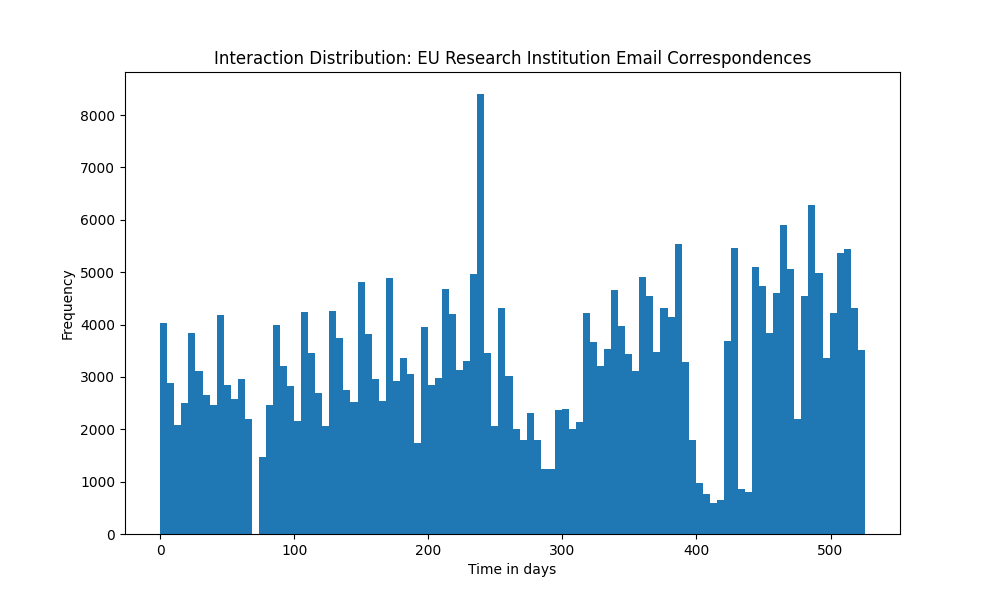
\includegraphics[width=\textwidth]{0_images/reallife_dataset_2_dist.png}
    \caption{A static graph representation of the relationships between characters in the book series 'Harry Potter'. Each node represents a specific character, that can be Hermione Granger, Ron Weasly or Harry Potter himself, and the edges that connect them represent the fact that a given pair of characters have interacted directly during the book series}
    \label{fig:StaticGraph}
\end{figure}


\subsubsection{Temporally Dynamic Graphs}
\label{sec:Method:Graphs:DynamicGraphs}
Not all networks can be represented by static graphs though, and sometimes having graphs be non-static means that they make for a better representation of the network they are modelling. 
When talking about temporally dynamic graphs, this project refers to graphs that are subject to a sequence of \textit{updates} over time. 
An update is an action that \textit{inserts} or \textit{deletes} edges or nodes in the graph or actions that \textit{alter attributes} of nodes or edges.


The dynamic aspect differ between graphs, as they can be changing in different dimensions. 
This project focuses entirely on the very commonly used graphs that are dynamic in the temporal dimension, \textit{temporal dynamics graphs}, i.e. they change over time, this is not always the case. 
Another example could be if we had a network representing the airports which a plane could directly fly to. 
Now the graph would be dynamic in the geographical position of the plane as the graph could change to show which airport the plane is connected to based on its current position. 
Say the graph for the plane being at the Reykjavik Airport on Iceland will then change when the plane gets to Los Angles.











\subsection{Latent Space Models}
\label{sec:Method:LSM}
This subsection delves into explaining and understanding the latent space modelling approach. A latent space, also refereed to as a latent embedding space, serves as an embedding in which a set of entities, in this project the nodes of a dynamic network, who resemble each other more closely are positioned closer in the latent space \cite{Sarkar2005DynamicModels} \cite{Kim2017AVariables}.
For a given set of four nodes, with weighted links between them, this weight can be represented in two-dimensional Euclidean latent space by their reciprocal distances.  

\begin{figure}[H]
    \centering
    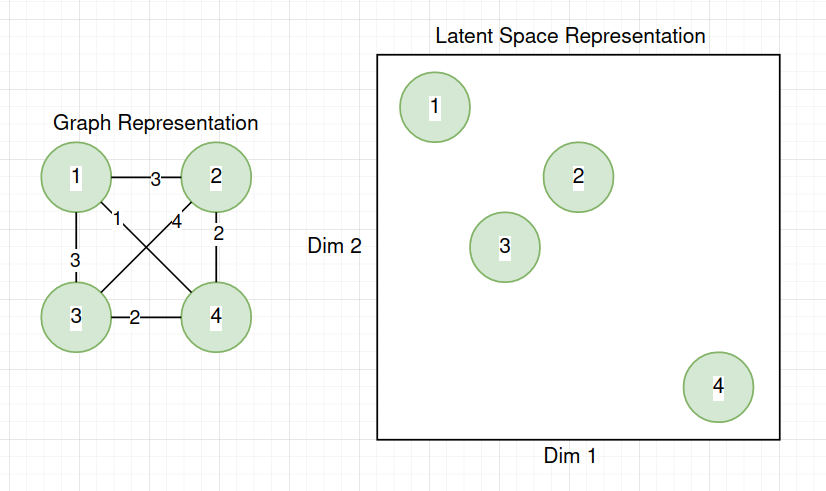
\includegraphics[width=0.8\textwidth]{0_images/latentspace.png}
    \caption{Four nodes placed in two-dimensional Euclidean latent space, weights represented by their reciprocal distances.}
    \label{fig:latentspace}
\end{figure}
\noindent
For this project, the resemblance of nodes, shown as the link weights in figure \ref{fig:latentspace}, is based on the intensity of interaction between entities in a given dynamic network.
This intensity is defined by the intensity function, which is described later in section \ref{sec:Method:IntensityFunc}.
\\
The latent space, being a two-dimensional space, serves as a dimensionality reduction, given the fact that the dynamics of the networks which are being mapped are of possibly much higher dimensions.
Latent space models, or latent distance models as they are also referred to, have proved good in modelling higher dimensional data in lower dimensions \cite{Gourieroux2021ScalableNetworks}.
As mentioned in section \ref{sec:Intro:RelatedWork} about related work, the latent space approach by Sarkar and Moore et. al. modelled dynamic networks using only positions in latent space \cite{Sarkar2005DynamicModels}.
Tomerup et. al. \cite{Tommerup2021LearningNetworks} expanded their modelling approach by attributing the nodes of a dynamic network with simple Newtonian dynamics of motion, and even though most dynamic networks are governed by Newtonian dynamics, this approach has the advantage of a higher degree of explainability.

\subsubsection{Euclidean Latent Space}
\label{sec:Method:LSM:EuclideanLatentSpace}
The 2D Euclidean latent space is governed by Euclidean geometry in two dimensions.
This means any measure of position, distance and velocity are understood as Euclidean and can be computed as such. 
Taking an offset in the nodes of a dynamic network, and the modelling approach presented in this project, the properties of Euclidean space will be explained below.
\\\\
Given a dynamic network consisting of $N$ nodes, these are all placed in Euclidean latent space. 
Positions in the Euclidean latent space are denoted as two-dimensional coordinates, and hence each node in the given network is assigned a position, expressed for node $u$ as
$$\textbf{z}_u = \begin{pmatrix}
x_u, y_u
\end{pmatrix}^T$$
\noindent
As the project deals with temporally dynamic networks specifically, the positions of nodes are temporally dependant. 
In order to accommodate for this, each node is assigned one or more velocity vectors, which entails that they move along the trajectory of a constant velocity over a given timespan.
For node $u$, the velocity vector is expressed as:
$$\textbf{v}_u = \begin{pmatrix}
v_{x,u}, v_{y,u}
\end{pmatrix}^T$$
\noindent
By having a starting position, $\textbf{z}_u$, as well as a constant velocity, $\textbf{v}_u$, the position of a node at any time, $t$, is given by: 

\begin{equation}
    \textbf{z}_u(t) = \begin{pmatrix}
    x_u\\
    y_u
    \end{pmatrix}
    +
    \begin{pmatrix}
    v_{x,u}\\
    v_{y,u}
    \end{pmatrix}
    t
    = 
    \begin{pmatrix}
    x_u + v_{x,u}t\\
    y_u + v_{y,u}t
    \label{eq:latent_pos}
    \end{pmatrix}
\end{equation}
In the Euclidean latent space, based on the given positions, it is possible to compute distances using basic Pythagorean mathematics. 
In order to find the distance between two nodes, the most straightforward approach is to compute their reciprocal Euclidean distance.
The distance at the starting position, i.e. disregarding time, between nodes $u$ and $v$, can be computed from the following expression:

\begin{equation}
    ||\textbf{z}_u - \textbf{z}_v||_2
    = 
    \sqrt{(x_u - x_v)^2 + (y_u - y_v)^2}
\end{equation}
As mentioned above though, the positions of nodes are in fact time dependant, and hence this carries over to the distance measure, which is expressed as:

\begin{equation}
    ||\textbf{z}_u(t) - \textbf{z}_v(t)||_2
    = 
    \sqrt{((x_u + v_{x,u}t) - (x_v + v_{x,v}t))^2 + ((y_u + v_{y,u}t) - (y_v + v_{y,v}t))^2}
\end{equation}
For mathematical and computational reasons, which are explained in detail under section \ref{sec:Method:IntensityFunc:IntegralIntensityFunc}, this project utilizes the squared Euclidean distance as distance measure.
This is written below, in a simplified form:

\begin{equation} 
||\textbf{z}_u(t) - \textbf{z}_v(t)||_2^2
= 
(x_u - x_v + (v_{x,u} - v_{x,v})t)^2 + (y_u - y_v + ( v_{y,u} - v_{y,v})t)^2
\label{eq:SquaredEuclideanDistance}
\end{equation}




\subsection{Poisson Distribution and Process}
\label{sec:Method:Poisson}
The Poisson distribution models the probability that a given number of independent events, from a discrete random variable, will happen in a specific time interval \cite{PoissonScience}. 
The events will happen at some rate, defined by the symbol $\lambda$, also named the intensity function. 
For instance, the Poisson distribution could model the discrete random variable that represents two nodes interacting, which can only take two values either 1 (interaction) or 0 (no interaction).
More formally the probability mass function of the Poisson distribution is described by:

\begin{equation}
    p_k = \frac{e^{-\lambda}\lambda^k}{k!} \;\; \text{for} \;\; \lambda > 0 \;\; \text{and} \;\; k = 0,1,\dots
\end{equation}
The intensity function might then be constant throughout the time interval or it may be time-dependent as a function of time, $\lambda(t)$.
Here, $k$ is the number of occurrences for a given event, in this case a node pair interacting and $p_k$ denotes the probability of getting $k$ occurrences.
Worth noting is that a random variable $X$, that is Poisson distributed with intensity rate $\lambda$, has $E[X] = \lambda = Var[X]$.


\subsubsection{Poisson Point Process}
\label{sec:Method:Poisson:PoissonPointProcess}
To understand the Poisson point process it is useful to first define the point process. 
A point process is a stochastic process with a collection of random variables that represent the arrival times of events i.e. when events happen. 
In the case of TDGNs this would be the time points when the nodes interact. 
These arrival times can be defined as ${t_n ; n \ge 0}$, such that:

$$
t_0 = 0 < t_1 < t_2 < ... < t_n
$$

where $t_n$ is the arrival time of the \textit{n}th event.
\\\\
Each of these arrival times will happen one after another, and the times between them are called interarrival times. 
They are independent random variables and can be defined for the point process as:

\begin{align*}
T_1 &= t_1 - t_0 \\
T_2 &= t_2 - t_1 \\
&\dots \\
T_n &= t_n - t_{n-1}
\end{align*}
where ${T_n ; n \ge 1}$ is a stochastic process with the random variables denoting the interarrival times.
\\\\
Now a Poisson point process with intensity, or rate, $\lambda > 0$ can be defined as a point process, where the interarrival times ${T_n ; n \ge 1}$ are independent exponentially distributed random variables. 
If the intensity function $\lambda$ of the Poisson process is constant for all time intervals, the process is said to be homogeneous. 
If the intensity function of the Poisson process is depending on time, i.e. $\lambda(t)$, then the process is said to be non-homogeneous or in-homogeneous.

In the case of this project a non-homogeneous Poisson point process is used. 
This is because the intensity function, which describes the likelihood of node interactions, is governed by the squared Euclidean distance between the nodes. 
This distance should change through time, as the nodes changes positions in the Euclidean latent space and as such the intensity function should change trough time \cite{Bas2019AProcess}.

During these interarrival times, the Poisson process increments happen as:

\begin{align*}
X_1 &= X(t_1) - X(t_0) \\
X_2 &= X(t_2) - X(t_1) \\
&\;\;\;\;\;\;\;\dots \\
X_n &= X(t_n) - X(t_{n-1})
\end{align*}
and are independent random variables that yield the number of events happening in the time interval $(t_{n-1}, t_n]$. 

Now if the Poisson process is homogeneous with $\lambda > 0$, has a starting time $s \ge 0$ and an interarrival time step $t > 0$, then the random variable $X(s+t) - X(s)$ is Poisson distributed, such that:

\begin{equation}
    P(X(s+t) - X(s) = k) = \frac{(\lambda)^k e^{-\lambda}}{k!} \;\; \text{for} \;\; k=0,1,\dots
\end{equation}
where $X(0) = 0$.

In the case of this project we are interested in the non-homogeneous Poisson process, in which case the process increments $X(s+t) - X(s)$ has the rate $\lambda(t)$ and becomes Poisson distributed with parameter $\int_s^t \lambda(u)\; du$, such that:

\begin{equation}
    P(X(s+t) - X(s) = k) = \frac{\left(\int_s^{s+t} \lambda(u) \; du \right)^k exp\left(-\int_s^{s+t} \lambda(u) \; du\right)}{k!}
\end{equation}
This gives the probability of having $k$ events in the time interval $(s, s+t]$ for the non-homogeneous Poisson point process.


\subsubsection{Event Probability}
\label{sec:Method:Poisson:EventProbability}
If we consider the case where the interarrival times $(s, s+t]$ are made infinitesimally small, such that $t = dt$, it will be assumed that no more than one event can occur during the interarrival time $(s, s+dt]$, leading to:

\begin{align}
P(X(s+dt) - X(s) = k) = 
\begin{cases}
    1 - \lambda(u) \; dt \; &\text{for} \; k=0 \\
    \lambda(u) \; dt \; &\text{for} \; k=1 \\
    0 \; &\text{for} \; k > 1
\end{cases}
\end{align}
This means that the event probability of a single event happening becomes:

\begin{align}
\begin{split}
    P(X(s+t) - X(s) = 1) 
    &= 
    \frac{\left(\int_s^{s+t} \lambda(u) \; du \right)^1 \exp \left(-\int_s^{s+t} \lambda(u) \; du\right)}{1!} \\
    &= 
    \left(\int_s^{s+t} \lambda(u) \; du \right) \exp \left(-\int_s^{s+t} \lambda(u) \; du\right)
\label{prob_single_event}
\end{split}
\end{align}
which can be rewritten, through the notion that for a function $f(x)$ with antiderivative $F(x)$ integrated over an infinitesimal interval it holds that:

\begin{equation}
    \int_s^{s+dt} f(u) \; du = F(u) \rvert_s^{s+dt} = F(s+dt) - F(s) = F^{\prime}(s) \; dst = f(s) \; dt
\end{equation}
Applied to (\ref{prob_single_event}), it yields:

\begin{equation}
    P(X(s+t) - X(s) = 1) = \lambda(s)dt \; e^{-\lambda(s)dt}
\end{equation}
This can be expanded with the power series to get:

\begin{equation}
    P(X(s+t) - X(s) = 1) = \lambda(s) dt
\end{equation}
Here, the higher orders of the infinitesimal $ds$ are neglected.


\subsubsection{Non-Event Probability}
\label{sec:Method:Poisson:NonEventProbability}
A similar starting point can be taken for the non-event probability as with the event probability.

If we consider the non-homogeneous Poisson point process with intensity $\lambda(t)$. 
The probability of no events happening during the interarrival time $(s, s+t]$ becomes:

\begin{equation}
    P(X(s+t) - X(s) = 0) 
    = 
    \frac{\left(\int_s^t \lambda(u)du \right)^0 \exp \left(- \int_s^t \lambda(u)du\right)}{0!}
    = 
    \exp \left(- \int_s^t \lambda(u)du\right)
\end{equation}
where $t = dt$ for infinitesimally small interarrival times.

\subsection{Intensity Function}
\label{sec:Method:IntensityFunc}
For the SCVM, an intensity function is defined for each pair of nodes in a given dynamic network.
The intensity function $\lambda_{u,v}$, governing the intensity of interaction between nodes $u$ and $v$, is written as the following:

\begin{equation}
    \lambda_{u,v}(t)
    =
    \exp \left(\beta - ||\textbf{z}_u(t) - \textbf{z}_v(t)||_2^2\right)
    \label{eq:IntensityFunc}
\end{equation}
This function is governed by two important terms.

The first, the distance term, is the reciprocal squared Euclidean distance of the node pair, which is described earlier in section \ref{sec:Method:LSM:EuclideanLatentSpace}.
This term is vital in reflecting the intensity of interaction between nodes as their reciprocal distance.
As the positions of nodes, and hence their reciprocal distances, are dependent on both starting positions and velocities, these are parameters the model will learn based ultimately on this intensity function.

The second term is the bias term $\beta$, a scalar which too is a learnable model parameter. 
The bias term serves as the background intensity and is hence used in modelling the intensity of interaction between nodes regardless of their reciprocal distances in Euclidean space. 
In this way, a large bias term will mean that nodes have higher intensity of interaction regardless of their latent positions and the opposite is true for a small bias term.


\subsubsection{Integral of the Intensity Function}
\label{sec:Method:IntensityFunc:IntegralIntensityFunc}
The intensity function for a given pair of two nodes, $u$ and $v$, using the bias term $\beta$ and squared Euclidean distance as distance term, is as stated above given by equation (\ref{eq:IntensityFunc}).
As seen earlier with equation (\ref{eq:SquaredEuclideanDistance}), the distance term can be written as a function of the starting position plus the velocity over time, and as such the node pair intensity function is given by:

\begin{equation}
    \lambda_{u,v}(t)
    =
    \exp \left(\beta - \left((x_u - x_v + (v_{x,u} - v_{x,v})t)^2 + (y_u - y_v + ( v_{y,u} - v_{y,v})t)^2\right)\right)
\end{equation}
In order to compute the log-likelihood, which is explained in the next section \ref{sec:Method:LikelihoodFunc}, the solution for the integral of the intensity function needs to be found. 

The reason the squared Euclidean distance is utilized, as opposed to using the standard Euclidean distance, is that it enables for an exact, analytical integration of the stated intensity function.
Having an analytical solution for the integral is important for this project, as it enables the computation to be exact and run fast, hence improving scalability.
This integral is written below:

\begin{equation}
    \int_{t_0}^{t_{n}} \lambda_{u,v}(s) \mathrm{d}s 
    =
    \int_{t_0}^{t_n} \exp \left(\beta - \left((x_u - x_v + (v_{x,u} - v_{x,v})s)^2 + (y_u - y_v + ( v_{y,u} - v_{y,v})s)^2\right)\right) \mathrm{d}s
\end{equation}
For ease of interpretation, substitutions are made for the following (without them, the final solution is incredibly long):

\begin{align}
    x_u - x_v &= a
    \\
    y_u - y_v &= b
    \\
    v_{x,u} - v_{x,v} &= m
    \\
    v_{y,u} - v_{y,v} &= n
\end{align}
This yields a substituted integral looking as such:

\begin{equation}
    \int_{t_0}^{t_n} \lambda_{u,v}(s) \mathrm{d}s 
    =
    \int_{t_0}^{t_n} \exp \left(\beta - \left((a + m \cdot s)^2 + (b + n \cdot s)^2\right)\right) \mathrm{d}s
\end{equation}
What is evident here, is that this integral must have an analytical solution, meaning conventional approximation approaches will not be needed in order to evaluate it's value. 
This is specifically due to the fact that the integration is happening over the exponential function of a function of quadratic form.

The analytical solution to this integral is computed as the following:

\begin{align}
    \int_{t_0}^T \lambda_{u,v}(s) \mathrm{d}s
    = 
    -\frac{\sqrt{\pi}}{2 \sqrt{m^{2}+n^{2}}}
    \cdot
    \exp\left(\frac{\left(-b^{2}+\beta\right) m^{2}+2abmn-n^{2}(a^{2}-\beta)}{m^{2}+n^{2}}\right)
    \\
    \cdot 
    \left(
    \operatorname{erf}\left(\frac{\left(m^{2}+n^{2}\right)t_{0}+am+b n}{\sqrt{m^{2}+n^{2}}}\right)
    -\operatorname{erf}\left(\frac{\left(m^{2}+n^{2}\right)T+am+b n}{\sqrt{m^{2}+n^{2}}}\right)
    \right)
    \label{eq:analytical_integral}
\end{align}
As can be seen above, the solution contains the Gauss error function denoted by $erf$.
This error function is a complex function of a complex variable, defined as:

\begin{equation}
\operatorname{erf} z=\frac{2}{\sqrt{\pi}} \int_{0}^{z} e^{-t^{2}} \mathrm{d} t
\end{equation}
What is important about the error function is that while it is in fact \textit{not} of a closed form, and hence disrupts the analytical nature of the integral, very efficient approximations can be made that eliminate the inconvenience of its non-closed form \cite{Ren2007Closed-formScience}.

\subsection{Likelihood Function}
\label{sec:Method:LikelihoodFunc}
In order to properly model a TDGN, the model presented in this project needs a metric on which it can train.
For this purpose, the likelihood function is introduced.
The likelihood function computes a metric on which the model optimization can be based, in this case relying heavily on the intensity function described above in section \ref{sec:Method:IntensityFunc}.
\\\\
This likelihood function computes the likelihood of the relevant input data, given a set of model parameters $\textbf{Z}$, $\textbf{V}$ and $\beta$.
In other words; with a set of model parameters, ie. the bias term $\beta$ as well as the starting positions $\textbf{Z}$ and constant velocities $\textbf{V}$ of the N nodes in the relevant TDGN, what is the likelihood that the input data, the chronologically ordered set of pairwise node interactions, would be occur/be produced.

For this project, the likelihood function, specifically the log-likelihood function, $\ell$ is given by the following expression:

\begin{equation}
    \ell = \sum_{i=1}^n \log \lambda (t_i) - \int_{t_0}^{t_n} \lambda(t) \mathrm{d} t
    \label{eq:LogLikelihoodFunc}
\end{equation}
This log-likelihood is given by the sum of the log of the intensity function for all interactions in the input data, $\sum_{i=1}^n \log \lambda (t_i)$, minus the integral of the intensity function, $\int_{t_0}^{t_n} \lambda(t) \mathrm{d} t$ \ref{sec:Method:IntensityFunc:IntegralIntensityFunc}, over the entire timespan and for all node pairs.

A more explicit way of writing the log-likelihood, while explicitly accounting for all node-pairs, is then.

\begin{equation}
    \ell = \sum_{i=1}^n \log \lambda_{u_i,v_i} (t_i) - \sum_{u=1}^{N-1} \sum_{v > u}^{N} \int_{t_0}^{t_n} \lambda_{u,v}(t) \mathrm{d} t
    \label{eq:LogLikelihoodFuncExplicit}
\end{equation}








\subsection{Proposed Model}
\label{sec:Method:ProposedModel}
The proposed model expands on the concept of a constant velocity model. Therefore this section will first introduce the constant velocity model as the base case for modelling node pair interactions, as presented by Simon Tommerup\cite{Tommerup2021LearningNetworks}. Then the actual proposed model, the stepwise constant velocity model, will be introduced as a more flexible way of modelling node pair interactions.  Finally it will be shown how the stepwise constant velocity model can be vectorized to make it scalable for use with frameworks like Pytorch and how regularization of the velocities in the stepwise model can be utilized to try and control the changes in the learned velocities from one step in the model to another, which is desirable for later visualizing the node movements in the latent space.


\subsubsection{Constant Velocity base Model}
\label{sec:Method:ProposedModel:ConstantVelocityModel}
The constant velocity model tries to determine the common bias term, initial position and initial velocity for N nodes in a TDGN, based on the pairwise node interactions happening over a given timespan.
\\\\
The model takes as input a chronologically ordered sequence of $n$ timestamped, pairwise node interactions, which are stored as $n$ tuples $(u_i, v_i, t_i)$.
Here, $u_i$ and $v_i$ denote the two interacting nodes for interaction $i$, and $t_i$ denotes the time of the interaction.
\\
The learnable parameters of the model are the set of parameter matrices $\textbf{Z}, \textbf{V} \in \mathbb{R} ^{N \times 2}$ as well as the bias term $\beta \in \mathbb{R}$.
The parameter matrix $\textbf{Z}$ contains starting positions for all $N$ nodes in the TDGN, holding the $x$-component in the first column, and the $y$-component in the second.
The same is true for $\textbf{V}$, just that it contains all node velocities, which hence are constant over the given timespan.
The bias term $\beta$, as explained in section \ref{sec:Method:IntensityFunc}, is a real number used in modelling the background intensity of interactions.
\\\\
Each pair of nodes, $u$ and $v$, are associated with a Poisson point process, described under section \ref{sec:Method:Poisson:PoissonPointProcess}.
These processes are each governed by an intensity function (\ref{eq:IntensityFunc}), described under section \ref{sec:Method:IntensityFunc}, which explains that the closer $u$ and $v$ are, the higher the intensity of interaction will be. 
These pairwise intensity functions are utilized in the log-likelihood function (\ref{eq:LogLikelihoodFuncExplicit}), described under section \ref{sec:Method:LikelihoodFunc}, which outputs the log-likelihood of the input data given the parameters of the model, matrices $\textbf{Z}$ and $\textbf{V}$, and the common bias $\beta$.
\\
The optimization problem of the model is to maximize the log-likelihood (in practice minimize the negative log-likelihood) of the input data by fitting the model parameters.
In this regard, the goal is to learn the true initial conditions, $\textbf{Z}, \textbf{V}, \beta$.

\paragraph{Latent Space Position Calculation}
Given a set of node pair interactions and the time of each interaction, the constant velocity model then calculates the latent space node position for a node $u$ at interaction time $t$ as:
\begin{equation}
    \textbf{z}_{u}(t) = 
    \begin{pmatrix}
        x_{u}(t) \\
        y_{u}(t)
    \end{pmatrix}
    =
    \begin{pmatrix}
        z_{u,x}+v_{u,x} \cdot t \\
        z_{u,y}+v_{u,y} \cdot t
    \end{pmatrix}
    \;\; , \;\; \textbf{z}_{u}(t)
    \label{eq:Method:ConstantVelocity:latent_pos}
\end{equation}
Where the subscripts $(u,x)$ and $(u,y)$ denotes the $x$ and $y$ dimension of node $u$.

\paragraph{Loss Function}
The loss function of the constant velocity model is comprised of two parts here named \textit{event intensity} and \textit{non-event intensity}. The event intensity is defined as the sum of intensities for all node pairs for each of their node interaction times in the input data. The non-event intensity is defined as the sum of intensities for all node pairs in the time span from 0 to the max time in the input independent of whether or not the node pairs have an event in the input data. 
The event intensity $I_e$ for an input of $n$ node pair interactions is calculated based on the sum of log intensities for each node pair which depends on the node pairwise distances according to the found latent space positions for each node pair at the time of their interaction computed in the constant velocity model as:
\begin{equation}
    I_e = \sum_{i = 0}^{n-1}  \lambda_{u_i , v_i}(t_i) =  \sum_{i =0}^{n-1} \beta - \rVert \textbf{z}_{u_i}(t_i) - \textbf{z}_{v_i}(t_i) \rVert_2^2
    \label{eq:Method:ProposedModel:event_intensity_calc}
\end{equation}
Where $\rVert \cdot \rVert_2^2$ is the squared Euclidean distance, $\beta$ is the common bias term, $\textbf{z}_{u_i , t_i}$ is the latent space position of node $u_i$ at interaction time $t_i$ as described in (\ref{eq:latent_pos}).
\\\\
The non-event intensity $I_n$ for $n$ node pair interactions is simply computed by directly implementing the analytical solution to the constant velocity intensity integral (\ref{eq:analytical_integral}) from section \ref{sec:Method:IntensityFunc:IntegralIntensityFunc} and summing over it for all node pairs using the model starting positions and velocities in $\textbf{Z}$ and $\textbf{V}$:
\begin{equation}
    I_n = \sum_{u=0}^{N-2} \sum_{v > u}^{N-1} \varphi_{u,v}(t_0,t_{max}) 
    \label{eq:Method:ProposedModel:nonevent_intensity_calc}
\end{equation}
Where $\varphi$ is the analytical solution to the constant velocity intensity integral evaluated for the start time $t_0=0$ and end time $t_{max}$ which is the latest node pair interaction time.
\\\\
The constant velocity model loss is then computed as
$$
\mathcal{L} = - I_e - I_n
$$
which is the negative log likelihood.

\subsubsection{Stepwise Constant Velocity Model (SCVM)}
\label{sec:Method:ProposedModel:PiecewiseConstantVelocityModel}

With the constant velocity model, it is possible to model interactions between $N$ nodes in a TDGN by finding their true starting positions and velocities, as well as the bias term $\beta$, for a given timespan.
\\\\
The positions of nodes are modelled to change, reflecting the change in intensity of interaction between nodes, starting in $\textbf{Z}$ at time $t=0$ and moving along the trajectories that result from the constant velocities $\textbf{V}$ over time, until end time $T$.
With only one set of parameters for the entire timespan of a TDGN, the modelling ability is limited to describing changes in intensity of interaction with only changes in positions, along the straight trajectories of the velocity vectors contained in $\textbf{V}$.
This will in many cases be insufficient for depicting the given TDGN in a useful manner. 
In order to model with greater detail, the Constant Velocity Model is therefore expanded to the Stepwise Constant Velocity Model (SCVM). 
The central idea with this model is to split the entire timespan of a TDGN into $S$ smaller time intervals where the node movements in each sub interval, or step, is modelled by a velocity vector. The model still relies on a single common bias term $\beta$, and a single set of node starting positions $\textbf{Z} \in \mathbb{R}^{N \times 2}$, but the velocity is expanded with another dimension $S$ corresponding to the number of steps, such that $\textbf{V} \in \mathbb{R}^{N \times 2 \times S}$.
Having several velocities should allow for the TDGN to be modelled in a much more detailed manner, and should result in better representations in the Euclidean latent space.
\\\\
This enables for an expansion of the visualization made in section \ref{sec:Method:VModel:ModellingApproach}, in which the TDGN was visually understood as nodes starting in one point and travelling on a straight path in Euclidean latent space.
Now, by having the nodes move according to the sequence of velocities contained in the SCVM, the nodes will be able to travel on non-linear paths through the Euclidean latent space.
The complexity of their movements will hence depend on the number of steps, $S$, with larger $S$ leading to more possible velocity changes.

\subsubsection{Model Step Size}
The model is given a notion of how much time a step in the $S$ dimension corresponds to which can be used to compute latent space node positions at specific time points. For simplicity the model assumes equal size for each step and that the start time is 0. Such that only a single step size is needed for the model:
\begin{equation}
    \Delta_{step} = \frac{t_{max}}{S}
\end{equation}
Where $t_{max}$ is the max time from the event interactions.

\paragraph{Latent Space Position Calculation}
\label{sec:Method:StepwiseLatentSpacePositions}
The idea of adding a step dimension to the velocity matrix means a slight change in how the latent node positions for each interaction time are computed. Expanding on the idea from the constant velocity position calculation (\ref{eq:Method:ConstantVelocity:latent_pos}) we add the notion of the model step size $\Delta_{step}$ and the extra dimension to $\textbf{V}$ of size $S$. 
We then define the latent space movement of a node $u$ to a time point t, with $0 < t \le t_{max}$, as the sum of movements from each step:
\begin{equation}
    \mathcal{M}_{u}(t) = \sum_{j = 1}^{S} \textbf{v}_{j, u} \cdot \Delta_{j}(t) \;\;,\;\; \mathcal{M}_{u} \in \mathbb{R}^2
\end{equation}
Where $\textbf{v}_{j,u}$ is the $j$'th step velocity for node $u$, and $\Delta_{j}(t)$ is the portion of $t$ that falls into step $j$ i.e.:
\begin{align}
    \Delta_{j}(t) = 
    \begin{cases}
        \Delta_{step} \;\; &\text{for} \;\; t \ge \Delta_{step} \cdot j\\
        \text{max}\left(0, t + \Delta_{step} - \Delta_{step} \cdot j\right) \;\; &\text{for} \;\; t < \Delta_{step} \cdot j
   \end{cases} \;\; , \;\; j \in \{1,2,...,S\}
\end{align}
\\
We then get the latent node position for a given node $u$ to time $t$ as:
\begin{equation}
    \textbf{z}_{u}(t) = 
    \begin{pmatrix}
        x_{u}(t) \\
        y_{u}(t)
    \end{pmatrix}
    =
    \begin{pmatrix}
        z_{u,x} + \mathcal{M}_{u,x}(t) \\
        z_{u,y}+ \mathcal{M}_{u,y}(t)
    \end{pmatrix}
    \;\; \text{for} \;\; \mathcal{M}_{u_i,x}(t) \;,\; \mathcal{M}_{u_i,y}(t) \in \mathbb{R}
    \label{eq:Method:ConstantVelocity:latent_pos}
\end{equation}
Which is similar to (\ref{eq:Method:ConstantVelocity:latent_pos}), but where $\mathcal{M}_{u,x}$ and $\mathcal{M}_{u,y}$ represent node $u$'s summed stepwise movements in the $x$ and $y$ direction from time 0 to time $t$.


\paragraph{Loss Function}
The loss function of the stepwise model loss function remains identical to that of the constant velocity model, since the event and non-event intensities $I_e$ and $I_n$ can still be calculated as in (\ref{eq:Method:ProposedModel:event_intensity_calc}) and (\ref{eq:Method:ProposedModel:nonevent_intensity_calc}). The only difference will be, that the latent space positions used to calculate the event intensities are computed using the method described in section \ref{sec:Method:StepwiseLatentSpacePositions}.


\subsubsection{Position Correction}
\label{sec:Method:ProposedModel:PositionCorrection}
Since the model is only fitted based on the relative node distances, and velocity changes if regularization is used. This means that the model is unaware of the exact values of the starting positions and velocities $\textbf{Z}$ and $\textbf{V}$ as long as the relative node distances produce a good fit. This also means that the model fitting can result in displacement from origo of the node starting positions and that drift can be introduced in the node positions, which is undesirable when visualizing the node behavior in latent space.
\\
But, it is possible to center the model and remove drift while preserving the model loss and there by produce a more understandable visualization. 
To center the node positions around origo the coordinate-wise mean of $\textbf{Z}$
\begin{equation}
        \overline{\textbf{z}} = 
    \begin{pmatrix}
        \overline{z}_x \\
        \overline{z}_y
    \end{pmatrix}
\end{equation}
is subtracted from the starting positions in $\textbf{Z}$. Then the squared Euclidean distance between a node pair becomes:
\begin{equation}
    \mathcal{D} =\rVert (\textbf{z}_u-\overline{\textbf{z}}) - (\textbf{z}_v-\overline{\textbf{z}}) \rVert_2^2 = 
    \rVert \textbf{z}_u - \textbf{z}_v \rVert_2^2 
\end{equation}
and stays unaffected.
\\\\
The same procedure is applied to the velocities $\textbf{V}$, which means that the node movement for a node $u_i$ now becomes:
\begin{align}
    \mathcal{M}_{u}(t) &= \sum_{j=1}^S \left[(\textbf{v}_{j,u} - \overline{\textbf{v}}_j) \cdot \Delta_{j}(t) \right] \\
    &= \sum_{j=1}^S \textbf{v}_{j, u} \cdot \Delta_{j}(t) - \sum_{j=1}^S \overline{\textbf{v}}_j \cdot \Delta_{j}(t)
\end{align}
For readability we define:
\begin{align}
    m_{u,1}(t) &=  \sum_{j=1}^S \textbf{v}_{j, u} \cdot \Delta_{j}(t) \\
    m_{u,2}(t) &= \sum_{j=1}^S \overline{\textbf{v}}_j \cdot \Delta_{j}(t)
\end{align}
The latent node position for node $u$ to time $t$ then becomes:
\begin{equation}
    \textbf{z}_{u}(t) = 
    \begin{pmatrix}
        x_{u}(t) \\
        y_{u}(t)
    \end{pmatrix}
    =
    \begin{pmatrix}
        z_{u,x} + m_{u,1,x}(t) - m_{u,2,x}(t) \\
        z_{u,y}+ m_{u,1,y}(t) - m_{u,2,y}(t)
    \end{pmatrix}
\end{equation}


\subsubsection{Extending Loss Function - Regularization of Velocity Changes}
\label{sec:Method:ProposedModel:Regularization}
The velocity from one step to another can change a lot. But, large changes in velocity can have a negative impact on the visualization of the node behavior in latent space e.g. if nodes dramatically speed up and down from step to step.
Therefore a regularization term is added to the model loss function which penalizes high changes in velocities from one step to the next:
\begin{align}
    \mathcal{L} = - \left((- I_e - I_n) + \gamma \sum_{i=1}^{S} \rVert \textbf{V}_i - \textbf{V}_{i-1} \rVert_{F}^{2}\right)
    \label{eq:Method:ProposedModel:vec_regularization}
\end{align}
Where $\gamma$ is the regularizatoin factor and $\rVert \cdot \rVert_F^2$ is the squared Frobenius norm.

\subsection{Scalability}
\label{sec:Method:Scalability}
A key focus of this project was to make the modelling approach scalable, in order to enable the modelling of larger, more realistic networks.
This subsection describes how vectorization of the model's calculations is introduced in order to parallelize the computations, enabling sufficient use of CUDA.

\subsubsection{PyTorch and CUDA}
\label{sec:Method:Scalability:PyTorch}
EXPLAIN THE MOST IMPORTANT PROPERTIES OF PYTOCH THAT MAKES VECTORIZATION SCALABLE



\subsubsection{SCVM Model Vectorization}
\paragraph{Vectorized Latent Space Position Calculation}
\label{sec:Method:LatentSpacePositionCalculation}
To compute the node intensities for the given node interactions in the training data, the model needs to find the positions of each node pair in the latent space at the time they interact. For this the model uses a $step$ function which takes as input a vector $\textbf{t} \in \mathbb{R}^{T}$ of $T$ \textit{unique} time points. Each time point $t_i$ in $\textbf{t}$ is then transformed into a vector $\boldsymbol{\Delta} \texfbf{t}_{i} \in \mathbb{R}^S$ of $S$ time delta values, where $S$ corresponds to the size of the Step dimension in the model velocity matrix $\textbf{V}$. The transformation from $t_i$ to $\boldsymbol{\Delta} \texfbf{t}_{i}$ is done by computing the portions of $t_i$ that falls into each step $s_j \in S$ such:
\begin{align}
    \boldsymbol{\Delta} \textbf{t}_{i-1,j-1} = 
    \begin{cases}
        \Delta_{step} \;\; &\text{for} \;\; t_i >= (\Delta_{step} \cdot j) \\
        \text{max}(0, t_i + \Delta_{step} - \Delta_{step} \cdot j) \;\; \;\; &\text{for} \;\; t_i < (\Delta_{step} \cdot j)
    \end{cases}
\end{align}
where $\boldsymbol{\Delta} \textbf{t}_{i,j}$ is the $j$'th entry of the $i$'th time delta vector and $i,i \in \{1,2,3,...,S\}$.
\\
From these delta time values and the model velocities it is possible to calculate node movements. The latent space node positions $\textbf{Z}_{t_i}$ for a given time $t_i$ can then be calculated as the latent starting positions $\textbf{Z}$ i.e. the positions at time 0, plus the cumulative sum of movements to the time point $t_i$:
\begin{align}
    \textbf{Z}_{t_i} = \textbf{Z}_{0} + \sum_{j=0}^{S-1}\textbf{V}_{j} \cdot \boldsymbol{\Delta} \textbf{t}_{i,j}
\end{align}
When this process is applied to all time points in $\textbf{t}$ we get a collection of latent position matrices $\textbf{Z}_t$ according to the number of time points i.e. $Z_t \in \mathbb{R}^{N\text{x}D\text{x}T}$, which can be used to compute the event intensity for each node pair interacting at each time point $t_i$.

\paragraph{Vectorized Loss Function}
DESCRIBE VECTORIZED EVENT AND NON-EVENT INTENSITIES, VECTORIZED REGULARIZATION AND COMBINE TO VECTORIZED LOSS FUNCTION.


\subsection{Poisson Point Process Simulation}
\label{sec:Method:PoissonSimulation}
This section is concerned with the topic of generating synthetic data.
Synthetic datasets are utilized in order to verify correct modelling performance, as it provides for ground truth metrics on which the trained model can be evaluated.


\subsubsection{Simulating the Non-Homogeneous Poisson process\cite{Ross2013GeneratingVariables}}
\label{sec:Method:PoissonSimulation:NonHomogeneous}
In order to generate synthetic data for the Stepwise model, the goal is to simulate all event times occurring in a Poisson process running from step start time $t_0$ to step end time $t_0 + \Delta_{step}$.
This is done by by generating succesive inter-arrival times, stopping when the sum of these exceed $t_0 + \Delta_{step}$.
The non-homogeneous Poisson process has the intensity rate function $\lambda(t)$, and uses the thinning method in which an upper bound $\lambda_U$ is determined.
The method finds an upper bound $\lambda_U$ that follows:

\begin{equation}
    \lambda(t) \leq \lambda_U \hspace{5pt} for \hspace{5pt} t \leq t_0 + \Delta_{step}
\end{equation}
It then simulates the event times for a homogeneous Poisson process with this upper bound intensity rate, $\lambda_U$, and 'thins' the events of this homogeneous Poisson process by accepting the event times with the probability given by:

\begin{equation}
    p_{accept}(t) = \frac{\lambda(t)}{\lambda_U}
\end{equation}
The remaining event times will follow the non-homogeneous Poisson process, as it is governed by the intensity rate function:

\begin{equation}
    \lambda_U \cdot p_{accept}(t) = \lambda_U \cdot \frac{\lambda(t)}{\lambda_U} = \lambda(t)
\end{equation}
In practise, this specific method of thinning will be rather inefficient, as alot of event times will be discarded, due to the fact that the intensity $\lambda(t)$ may vary greatly over the given timespan $t_0$ to $t_0 + \Delta_{step}$.
To accommodate for this, the time interval is split into $k$ smaller sub-intervals:

\begin{equation}
    t_0 < t_1 < \dots < t_{k+1} = t_0 + \Delta_{step}
\end{equation}
Each of these are given an upper bound, ie.:

\begin{equation}
    \lambda_{U,1}, \dots, \lambda_{U,k+1}
\end{equation}
For which it is given that:

\begin{equation}
    \lambda(s) \leq \lambda_{U,i} \hspace{5pt} if \hspace{5pt} t_{i-1} \leq s \leq t_i \hspace{5pt} for \hspace{5pt} i = 1,\dots,k+1
\end{equation}
\\
The general algorithm for simulating a non-homogeneous Poisson process with rate $\lambda(t)$, utilizing these principles, is then given by:

\begin{figure}[H]
    \centering
    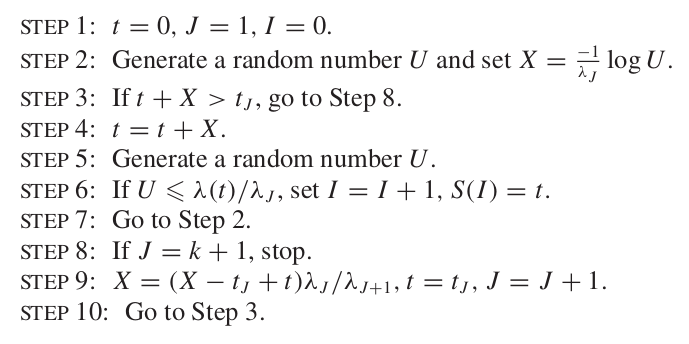
\includegraphics[width=0.6\textwidth]{0_images/nonHomogeneousAlgorithm.png}
    \caption{General non-homogeneous Poisson process simulation algorithm .}
    \label{fig:NonHomogeneousGeneralAlgorithm}
\end{figure}


\subsubsection{Stepwise Model Modified Simulation}
\label{sec:Method:PoissonSimulation:NonHomogeneousModified}
In the case of this project, the aforementioned intensity function $\lambda(t)$ is governed by the 2D squared Euclidean distance between a given pair of nodes $(u,v)$, explained in section \ref{sec:Method:IntensityFunc}, and given by:

\begin{equation}
    \lambda_{u,v}(t)
    =
    \exp \left(\beta - ||\textbf{z}_u(t) - \textbf{z}_v(t)||_2^2\right)
    \label{eq:IntensityFunc2}
\end{equation}
\noindent
First of all, this means that for each time step ranging from $t_0$ to $t_0 + \Delta_{step}$, the non-homogeneous Poisson process has to be simulated for each of $\frac{N(N-1)}{2}$ node pairs.
\noindent
Secondly, finding the upper bound $\lambda_U$ of a given intensity function $\lambda_{u,v}(t)$ is not straight forward, as the different intensity functions may either be descending or ascending in the given step's time interval, and have a local minimum or maximum.
The explained method for simulating a non-homogeneous Poisson process using thinning is therefore slightly modified in order to accommodate for this difficulty.
\\
For each node pair in each step, the monotonicity of the intensity function is found from looking at the sign around the roots of the derivative solved for zero of the intensity function.
For each step and node pair, the aforementioned $k$ time sub-intervals are now mapped along this found monotonicity, keeping track of where the roots of the solved intensity function derivative are in relation to each sub-interval.
This means that a given sub-interval for time $[t_n,t_{n+1}]$ has the monotonicity corresponding to the sign of the derivative $\frac{d}{dt} \lambda_{u,v}(t)$ when between two roots.
If the sign is negative, i.e. the monotonicity is decreasing, the upper bound intensity rate is set to $\lambda_U = \lambda_{u,v}(t)$.
If the monotonicity is increasing, the upper bound is set to $\lambda_U = \lambda_{u,v}(t+1)$.
In the cases the monotonicity changes from positive to negative for the next sub-interval, i.e. passing a local maximum, the current sub-interval is positioned over a root, and gets the upper bound of $\lambda_U = \lambda_{u,v}(r)$.
If the monotonicity changes from negative to positive, the sub-interval is placed over a local minimum root, and must get the upper bound $\lambda_U = \text{max}(\lambda_{u,v}(t_n), \lambda_{u,v}(t_{n+1}))$

%\subsection{Model Implementation}
%\label{sec:Method:ModelImplementation}
%The proposed model is implemented using \hyperlink{https://pytorch.org/docs/1.9.1/}{Pytorch-1.9.1}\cite{PyTorchDocumentation} and contains the learnable parameters, $\textbf{z0} \in \mathbb{R}^{N \times 2}$, $\textbf{v0} \in \mathbb{R}^{N \times 2}$ and $\beta$. Here $\beta$ is a scalar representing the common bias term, $\textbf{z0}$ and $\textbf{v0}$ are tensors where $N$ is the number of unique nodes in the TGDN, $D$ is the size of the latent Euclidean space, which is chosen to be 2 for a 2-D latent space visualization of the TDGN, and $S$ is the number of steps in the model e.g. if the model tries to learn a representation, where the velocity can change 4 times, then S = 4.



% \subsection{Learning}
% \label{sec:Method:Learning}
% This section briefly describes the learning setup for the proposed model.
% The model learning is implemented using the \hyperlink{https://pytorch.org/ignite/}{Pytorch-Ignite-0.4.7}\cite{IgniteDocumentation} framework.
%  %The model training uses batching to handle the large amounts of data for TDGNs with many interactions. where each batch fed to the model contains $E$ rows for $E$ node interactions and 3 columns . which are fitted using backpropagation, based on the negative of the loglikelihood presented in equation  \ref{eq:LogLikelihoodFuncExplicit} in section \ref{sec:Method:LikelihoodFunc}










\subsection{Model Evaluation}
\label{sec:Method:Evaluation}
In order to evaluate the performance of the models presented in this project, hence verifying they work as intended, they are evaluated on synthetically generated data. 
This data, which is generated based on chosen parameters $\beta$, $z0$ and $v0$ allows for the existence of a ground truth model with metrics which a given trained model should converge towards. 

The essence of the model evaluation is verifying that a trained model has modelled a given TDGN correctly, even though is has not found the same $z0$ and $v0$ as the synthetic dataset is generated from.
This is important, as there in theory is an infinite set of correct initial parameters, which yield a correctly modelled TDGN. 
Intuitively, initial parameters (\ref{eq:InitParam1}) and (\ref{eq:InitParam2}) below will yield (almost) identical datasets.

\begin{align}
    z0 &= \left( \begin{matrix}
                0.0 & 1.0\\
                0.0 & -1.0\\
                \end{matrix}\right), \hspace{10}
    v0 = \left( \begin{matrix}
                0.0 & -0.01\\
                0.0 & 0.01\\
                \end{matrix}\right), \hspace{10}
    \beta = 7.5
    \label{eq:InitParam1}
    \\
    z0 &= \left( \begin{matrix}
                1.0 & 0.0\\
                -1.0 & 0.0\\
                \end{matrix}\right), \hspace{10}
    v0 = \left( \begin{matrix}
                -0.01 & 0.0\\
                0.01 & 0.0\\
                \end{matrix}\right), \hspace{10}
    \beta = 7.5
    \label{eq:InitParam2}
\end{align}


\subsubsection{Baseline Models}
\label{sec:Method:Evaluation:BaselineModels}
Baseline models will be utilized in order to evaluate wheter the proposed model is an improvement over prior work.

There are three baseline models, which are incrisingly complex in their modelling capability.
\\\\
The first baseline consists in modelling the data by taking the average intensity of the nodepairs.
\\\\
The second baseline is the Constant Velocity model withour velocity, ie. merely fitting nodes to the optimal positions, but not attributing them a velocity.
\\\\
The third baseline used is the one-step Constant Velocity model.
For modelling synthetic dataset 1 which is generated from a single velocity vector, see section \ref{sec:Method:Reproducibility:SyntheticDataset1}, this baseline will be redundant.
For either synthetically generated data on more steps, or real data, this baseline will fit only one velocity for each node, one step.


\subsubsection{Beta Convergence}
\label{sec:Method:Evaluation:BetaConvergence}
A properly trained Constant Velocity Model, which correctly models the given TDGN, most likely does not find the same parameters $z0$ and $v0$ as that of the ground truth model.
It should, however, find a $\beta$-value close to the ground truth, as this parameter strongly governs the intensity of interaction between nodes, as of the intensity function (\ref{eq:IntensityFunc}):
\begin{equation*}
    \lambda_{u,v}(t)
    =
    \exp \left(\beta - ||\textbf{z}_u(t) - \textbf{z}_v(t)||_2^2\right)
\end{equation*}
Hence, a strong indication of good modelling consists in whether $\beta$ converges correctly.


\subsubsection{Average Training Loss}
\label{sec:Method:Evaluation:Loss}
The loss, ie. negative log likelihood computed during model training, see section \ref{sec:Method:LikelihoodFunc}, gives a clear picture of model training progress.
In this project, the average loss, meaning loss over the number of interactions in the given dataset, is used as it represents a more similar metric across different datasets.
\\
The average loss is written as:

\begin{equation}
   average loss = - \frac{\ell}{n_{dyads}} = - \frac{\sum_{i=1}^n \log \lambda_{u_i,v_i} (t_i) - \sum_{u=1}^{N-1} \sum_{v > u}^{N} \int_{0}^T \lambda_{u,v}(t) \mathrm{d} t}{n_{dyads}}
    \label{eq:LogLikelihoodFuncExplicit}
\end{equation}
When training on synthetic data, the present ground truth model enables for the computation of a ground truth average loss, to which the trained model should preferably converge.


\subsubsection{Intensity Rate Comparison}
\label{sec:Method:Evaluation:Intensity}
The interaction intensity between a given pair of nodes, over the temporal span of the TDGN, can be inspected accurately and serves as a more visual comparison to the GT model than the loss. 
While using the average loss as a metric essentially enables for comparing the altogether deviation between the ground truth model and the learned model, singling out node pairs can better the understanding of a good fit for TDGN's with few nodes.




\subsubsection{Node Pair Removal}
\label{sec:Method:Evaluation:NodePairRemoval}
Building on top of intensity rate comparison for node pairs, a very concrete test of modelling performance and to some extend modelling stability is devised.
For a given TDGN consisting of $N$ nodes, with a dataset consisting of interactions between $\frac{N\cdot(N-1)}{2}$ pairs of nodes (assuming they all interact), a fraction of about 10\% of the node pairs, or dyads as they may be called, are removed from the dataset before training.
After training, the modelled intensity of interaction is compared with the ground truth, revealing how well the model is able to model the TDGN with entirely missing dyads, and to some extend how well it is able to infer the interactions of removed dyads based solely on their non-removed counterparts.


\subsubsection{AUC Score of Removed Interactions}
\label{sec:Method:Evaluation:AUC}
In order to test the model on real data, a test which does not require a ground truth model is devised.
From the dataset, 10\% of interactions are removed before training.
For each time point in the removed interactions, an alternative, false interaction is sampled, and the model is posed with evaluating the probability of the real interaction contra the false one.
The probability is computed as the log of the event probability, explained under section \ref{sec:Method:Poisson:EventProbability}.

The AUC score is computed as the area under the ROC (Receiver Operating Characteristics) curve.
The ROC curve is the False Positive rate vs. the True Positive rate at some given decision thresh holds.




\clearpage

\section{Data}
\label{sec:Data}
In order to enforce reproducibility of results, this section provides a detailed description of the setup used in order to generate the synthetic data utilized in the results section, as well as the real datasets.

\subsection{Synthetic Data}
\label{sec:Data:SyntheticData}
The synthetic data used for validating the Constant Velocity Model is generated in order to be in possession of a ground truth set of parameters with which the model can be evaluated.
Mathematically, the data is based int the Poisson process explained in detail under section \ref{sec:Method:Poisson}.

The ground truth parameters that need to be determined are how many nodes $N$ are in the desired system, their initial positions $Z$, their initial velocities $V$ and the $\beta$ background intensity.
One further parameter that has to be determined is the max time with which interactions are counted in, meaning interactions of time $t > t_{max}$ are not included in the synthetic dataset.


\subsubsection{Synthetic Dataset 1}
\label{sec:Data:SyntheticData:SyntheticDataset1}
The first synthetic dataset is small, consisting of four nodes, and will only be utilized in order to evaluate the Constant Velocity Model in a one-step setting.

The ground truth parameters of the first synthetic dataset are as follows:
\begin{equation}
    N = 4, \hspace{10}
    t_{max} = 10, \hspace{10}
    Z = \left( \begin{matrix}
                -0.6 & 0.0\\
                0.6 & 0.1\\
                0.0 & 0.6\\
                0.0 & -0.6
                \end{matrix}\right), \hspace{10}
    V = \left( \begin{matrix}
                0.09 & 0.01\\
                -0.01 & -0.01\\
                0.01 & -0.09\\
                -0.01 & 0.09
                \end{matrix}\right), \hspace{10}
    \beta = 7.5
\end{equation}
These ground parameters yield a dataset, tuples denoting the two interacting nodes $u$ and $v$ as well as the time of interaction $t$, ie. $(u_i, v_i, t_i)$, which has size $n=79,424$.


\subsubsection{Synthetic Dataset 2}
\label{sec:Data:SyntheticData:SyntheticDataset2}
The second synthetic dataset is utilized in order to test the modelling capabilities of the stepwise Constant Velocity Model. 

In order to generate a dataset which has attributes that make sense modelling using a stepwise approach, the velocities of the nodes is changed over the timespan from 0 to $t_{max}$.
For synthetic dataset 2, five nodes are each attributed a starting position and 10 velocity vectors.

The ground truth parameters of the second synthetic dataset are as follows:
\begin{equation}
    N = 5, \hspace{10}
    t_{max} = 50, \hspace{10}
    Z = \left( \begin{matrix}
                1 & 1\\
                1 & -1\\
                -1 & 1\\
                -1 & -1\\
                0 & 2
                \end{matrix}\right), \hspace{10}
    V_1 = \left( \begin{matrix}
                -0.15 & -0.15\\
                -0.15 & 0.15\\
                0.15 & -0.15\\
                0.15 & 0.15\\
                0.05 & -0.3
                \end{matrix}\right)... 
    V_{10} = \left( \begin{matrix}
                -0.15 & 0.05\\
                -0.15 & -0.05\\
                0.15 & -0.05\\
                0.15 & 0.05\\
                0.1 & 0.05
                \end{matrix}\right), \hspace{10}
    \beta = 7.5
\end{equation}
These ground parameters yield a dataset which has size $n=330,023$.



\subsubsection{Synthetic Dataset 3}
\label{sec:Data:SyntheticData:SyntheticDataset3}
The third synthetic dataset is utilized in order to test scalability of the model, and for this purpose it is changeable in terms of number of nodes and beta value.
The number of nodes is chosen from the following range of $N$'s:
\begin{equation}
    N = [2, 4, 6, 8, 10, 12, 14, 16, 18, 20, 22, 24, 26, 28, 30, 34, 38, 42, 46, 50, 60]
\end{equation}
For the dataset consisting of $N = 2$ nodes, the starting positions are:
\begin{equation}
        Z = \left( \begin{matrix}
                1.0 & 0.0\\
                -1.0 & 0.0\\
                \end{matrix}\right)
\end{equation}
For the dataset consisting of $N = 6$ nodes, four more nodes are added which are placed further up along the y-axis, as the following:
\begin{equation}
        Z = \left( \begin{matrix}
                1.0 & 0.0\\
                -1.0 & 0.0\\
                1.0 & 1.0\\
                -1.0 & 1.0\\
                1.0 & 2.0\\
                -1.0 & 2.0\\
                \end{matrix}\right)
\end{equation}
The beta value $\beta$ is, like the number of nodes, also chosen from a range as follows:

\begin{equation}
    \beta = [5.0, 5.25, 5.5, 5.75, 6.0, 6.25, 6.5, 6.75, 7.0, 7.25, 7.5, 7.75, 8.0, 8.25, 8.5, 8.75, 9.0]
\end{equation}
The max time is $t_{max} = 20$, and as such the remaining ground truth parameter of the third synthetic dataset is the velocities of the four steps, which are replicated for each added set of nodes:
\begin{equation}
    
    V_1 = \left( \begin{matrix}
                -0.2 & -0.05\\
                0.2 & 0.05\\
                \end{matrix}\right), \hspace{5}
    V_2 = \left( \begin{matrix}
                0.2 & 0.05\\
                -0.2 & -0.05\\
                \end{matrix}\right), \hspace{5}
    V_3 = \left( \begin{matrix}
                -0.3 & -0.05\\
                0.3 & 0.05\\
                \end{matrix}\right), \hspace{5}
    V_4 = \left( \begin{matrix}
                0.3 & 0.05\\
                -0.3 & -0.05\\
                \end{matrix}\right)
\end{equation}


\subsection{Real Data}
\label{sec:Data:RealData}


\subsubsection{Real Dataset 1: Player Interactions in a game of 'Resistance'}
\label{sec:Data:RealData:RealDataset1}
Dataset can be found here: \href{https://snap.stanford.edu/data/comm-f2f-Resistance.html}{https://snap.stanford.edu/data/comm-f2f-Resistance.html}
\\\\
The first real-life dataset consists of player interactions in a game of Resistance.

The Resistance game is a discussion, find-the-fraudster game, in which each player has a role belonging to either the resistance (good guys) or government spies (evil guys).
Only the government spies know the identity of their teammates, and so the goal of the game is for the resistance to identify the spies through verbal communication and vote them out, while the spies try to vote out the resistance by convincing their opponents of their innocence. 
The interactions they make consist in one player addressing another player verbally, and the eight most clear interactions have been recorded for each timestep, which consist in thirds of a second. 
The players can also address the computer for hints, but it cannot address the players.

The specific dataset, game 4 of the included 62 games in the dataset, has eight players and a computer, ie. nine nodes, making 58.584 interactions spanning from time $t_{min} = \frac{0}{3}$ seconds to $t_{max} = \frac{7322}{3}$ seconds, approximately $40$ minutes and $40$ seconds.

The timestamps are transformed from thirds of a second to minutes by the following formula:

\begin{equation}
    t_i = 40.67 \cdot \frac{t_i - t_{min}}{t_{max}}
\end{equation}
The overall distribution of interactions are completely uniformly distributed due to the recording process.



\subsubsection{Real Dataset 2: EU Research Institution Email Correspondences}
\label{sec:Data:RealData:RealDataset2}
Dataset can be found here: \href{https://snap.stanford.edu/data/email-Eu-core-temporal.html}{https://snap.stanford.edu/data/email-Eu-core-temporal.html}
\\\\
The second real-life dataset consists of email correspondences between institution members.
The original dataset consists of 332.334 member-interactions (email exchanges) timestamped in seconds, with the first email being sent at time $t_{min} = 0$ seconds and the last email being sent at 69.459.254 seconds, 803 days after the first.
The dataset is reduced to 329.910 interactions due to a large empty gap between times $5 \cdot 10^5$ seconds and $6.88 \cdot 10^5$ seconds, whereas the last 2424 interactions are removed, hence the max time is $t_{max} = 45,405,138$ second, approximately 525.52 days.

The timestamps are transformed to days by the following formula:

\begin{equation}
    t_i = 525.52 \cdot \frac{t_i - t_{min}}{t_{max}}
\end{equation}
The distribution of email exhanges are as seen below in figure \ref{fig:RLdataset2}:

\begin{figure}[H]
    \centering
    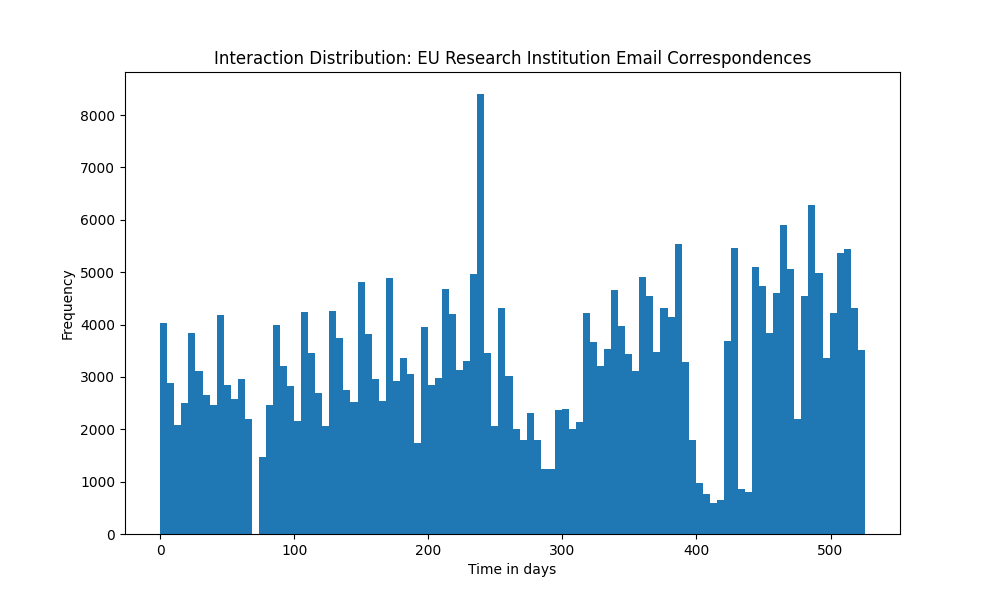
\includegraphics[width=\textwidth]{0_images/reallife_dataset_2_dist.png}
    \caption{Distribution of Real Dataset 2: EU Emails}
    \label{fig:RLdataset2}
\end{figure}


\subsubsection{Real Dataset 3: Student interactions in Lyon Primary School}
\label{sec:Data:RealData:RealDataset3}
Dataset can be found here: \href{http://www.sociopatterns.org/datasets/co-location-data-for-several-sociopatterns-data-sets/}{http://www.sociopatterns.org/datasets/co-location-data-for-several-sociopatterns-data-sets/}
\\\\
The third real-life dataset consists of co-location data of the students and teachers of a primary school in Lyon, France.
The original dataset consists of 241 individuals with 6.594.492, 20-second co-locations, meaning face-to-face interactions that persist over the span of 20 seconds.
The first interactions happening at $t_{min} = 34,240$ seconds and the last at 151.960 seconds.
The data is essentially split in two, temporally, and around half of interactions, 3.510.605, happen before time $t_{max} = 65,840$ seconds.
The dataset used for the project is this first half, consisting of $N = 237$ nodes with $n = 3,510,605$ interactions.
%From this half, the $n = 958,220$ interactions of 98 students and teachers are utilized.

The timestamps are transformed to hours, starting at hour 0 and ending at 84.25, by the following formula:

\begin{equation}
    t_i = \left(\frac{t_{max} - t_{min}}{3 \cdot 60} \right) \cdot \frac{t_i - t_{min}}{t_{max}}
\end{equation}
The distribution of these interaction have the distribution shown in figure \ref{fig:RLdataset3} below:

\begin{figure}[H]
    \centering
    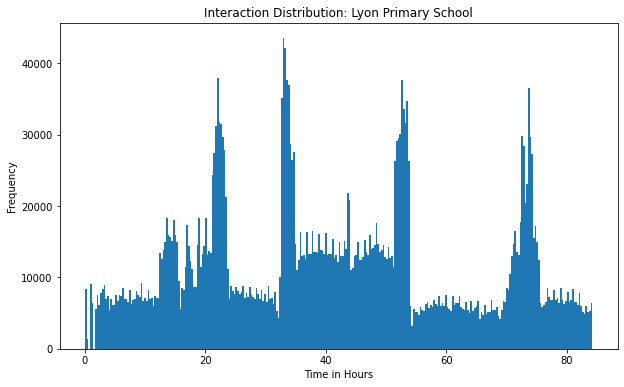
\includegraphics[width=\textwidth]{0_images/real_dataset_3_dist.png}
    \caption{Distribution of Real Life Dataset 3: Lyon Primary School}
    \label{fig:RLdataset3}
\end{figure}








\clearpage

\section{Results}
\label{sec:Results}
This section presents results that are used in answering the stated research questions.
\subsection{Training Setup and Hyperparameters}
\label{sec:Method:Reproducibility:TrainingSetup}
The proposed model, as well as baseline models, are governed by several hyperparameter options that naturally changes result-outcomes. 
\\\\
Training the models in this project is done using the Adam optimization algorithm, short for Adaptive Moment Estimation, which is a form of stochastic gradient descent \cite{Kingma2014Adam:Optimization}.
% A gradient descent algorithm seeks to optimize learnable parameters by stepping towards the direction of the negative gradient of the loss function with respect to these parameters.
% This way, the model will eventually find the parameters that, globally or locally, minimize the loss function.
% What makes the Adam optimization a stochastic gradient descent is the fact that the gradient is a stochastic approximation of the gradient based on the given batch of training data.
The most important hyperparameter in regards to the Adam optimization algorithm is the learning rate, usually denoted by $\alpha$, which determines the step size that is taken in the direction of the negative gradient. 
%As Adam builds upon the RMSProp optimizer, short for Root Mean Square Propagation, this learning rate is adapted for each learnable parameter, and hence slightly changing.

For this project, a learning rate of $lr = 0.025$ was found to be a good fit as it converges relatively quickly while not overshooting for most trainings.
Other hyperparameters of the training setup is Pytorch default.

Note that all random number generators in this project, belonging to Python, Numpy and Torch, are set to $seed = 1$.

While the number of Epochs needed by the SCVM for properly learning different dynamic networks, the proposed model could in most cases train for 5000 epochs in at most a couple of hours.
5000 epochs was enough for all trainings to seemingly converge.




%%%%%%%%%%%%%%%%%%%%%%%%%%%%%%%%%%%%%%%%%%%%%%%%%%%%%%%%%%%%%%%%%%%%%%%%%%%%%%%%%%%%%%%%%%
\subsection{First Research Question}
\label{sec:ResearchQuestion1}

\clearpage
\subsection{Second Research Question}
\label{sec:ResearchQuestion2}
The second research question of this project states:
\\
"To what extend can the model be implemented in a scalable manner?"
\\\\
In order to answer this research question, two overall experiments will be conducted.
First the proposed vectorized SCVM will be compared to a baseline model followed by an experimental investigation of the run time for the SCVM in relation to number of nodes, number of steps and number of interactions.
\\\\
The hardware used for testing is a Dell XPS-15-7590, with the following specifications:
\\
Ubuntu 20.04.3 LTS, 64-bit.
\\
16 Gigabyte RAM.
\\
CPU: Intel Core i7-9750H CPU @ 2.60GHz × 12.
\\
GPU: NVIDIA Corporation TU117M [GeForce GTX 1650 Mobile / Max-Q].


\subsubsection{Baseline Non-Vectorized vs. Vectorized Model Training}
\label{sec:ResearchQuestion2:BaselineComparison}
The proposed SCVM presented in this project utilizes vectorization in order to parallelize computation for model training.
In order to evaluate the improvement this entails over previous work, namely the CVM proposed by Tommerup et. el. \cite{Tommerup2021LearningNetworks}, the run times and memory requirements for training on a dynamic, one-step network with an increasing number of (few) nodes is evaluated.

Below, table \ref{tab:RuntimeBaseline} shows the run times for the baseline model, non-vectorized SVM, and the proposed model, vectorized SCVM, trained for 500 epochs on the first two, three and all four nodes of synthetic dataset 1 (see sections \ref{sec:Data:SyntheticData:SyntheticDataset1}).
The models were trained on the CPU.

\begin{table}[H]
\centering
\begin{tabular}{|l|ccc|}
\hline
Model           & \multicolumn{1}{l}{2 Nodes ($n = 11,133$)} & 3 Nodes ($n = 39,546$)& 4 Nodes ($n = 79,424$)         \\ \hline
Baseline CVM    & X                         & X             & 2h 52m 53s: 10,373s    \\
Vectorized SCVM & 2m 18s: 138s              & 3m 17s: 197s  & 5m 19s: 319s    \\ 
Run time improvement & $X$ times faster             & $X$ times faster  & $32.5$ times faster   \\ \hline
\end{tabular}
\caption{Run times for the non-vectorized CVM vs. the vectorized SCVM}
\label{tab:RuntimeBaseline}
\end{table}
\noindent As can be seen in table \ref{tab:RuntimeBaseline} above, the improvement in computational speed is beyond drastic.
The baseline model, when compared to the vectorized SCVM proposed in this project, takes a tremendous amount of time in order to train on a relatively small dataset.



\subsubsection{Computation Speed of the Proposed SCVM}
\label{sec:ResearchQuestion2:ComputationSpeed}
In order to evaluate the scalability of the proposed SCVM, the run times are evaluated in relation to the number of nodes in a given dynamic network, the number of interactions in a given dynamic network, and the number of steps the model has to fit to the data.

For these tests, synthetic dataset 3, see section \ref{sec:Data:SyntheticData:SyntheticDataset3}, is utilized.
This dataset is setup as to be changeable in terms of number of nodes $N$ and the bias term/beta value $\beta$ influencing the number of interactions generated.
\\\\
\textbf{Number of Nodes $N$}
\\
The first test which is carried out is for evaluating the impact increasing the number of nodes has on the run time of the SCVM.
For this test, the number of nodes is taken from the range:
\begin{equation}
    N = [2, 4, 6, 8, 10, 12, 14, 16, 18, 20, 22, 24, 26, 28, 30, 34, 38, 42, 46, 50, 60]
\end{equation}
The dataset is generated using $\beta = 5.0$ and four steps, ie. velocity vectors, are learned by the SCVM.
As increasing the number of nodes naturally increases the number of interactions, ie. the size of the dataset, and this test seeks to evaluate \textit{only} the impact that $N$ has on the run time, $n = 10,000$ interactions are used for all number of nodes.

For each $N$, five trainings of 10 epochs are carried out and the mean of their training times are recorded.
These means are divided by the number of epochs run, 10, hence yielding the mean run time per epoch for a given number of nodes.
This is done using both the CPU and the GPU (CUDA).

Figure \ref{fig:NumNodesRuntimes} below shows the run times per epoch given the number of nodes, using the CPU (in blue) and CUDA (in orange).

\begin{figure}[H]
    \centering
    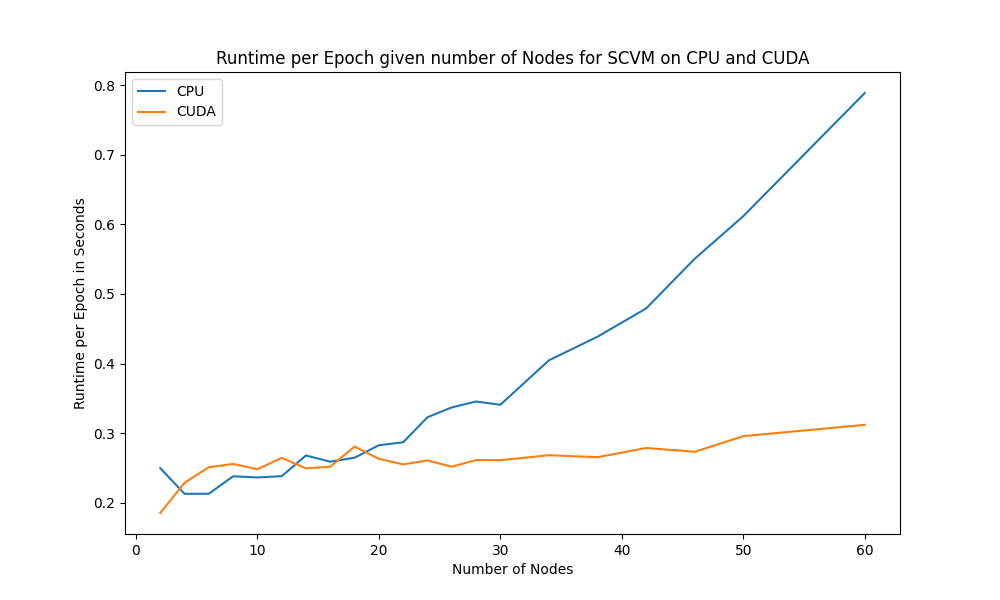
\includegraphics[width=\textwidth]{0_images/numnodes_runtime2.png}
    \caption{Run time of the SCVM relative to the number of nodes $N$}
    \label{fig:NumNodesRuntimes}
\end{figure}
\textbf{Number of Steps}
\\
The second test is carried out in order to evaluate the impact on run time in relation to the number of steps the SCVM has to fit.
For this test, the number of steps is taken from the range:
\begin{equation}
    Num\_Steps = [4,8,12,16,20,30,40,50,75,100,150,200,250,300,350,400,450,500,750,1000]
\end{equation}
The dataset is generated using $\beta = 5.0$ and $N = 4$ nodes, and the resulting dataset has size $n = 5997$.
Again, for each number of steps, the mean run time per epoch over five runs are recorded for both the CPU and CUDA.

Figure \ref{fig:NumStepsRuntimes} below shows the run times per epoch given the number of steps the SCVM has to fit, using the CPU (in blue) and CUDA (in orange).

\begin{figure}[H]
    \centering
    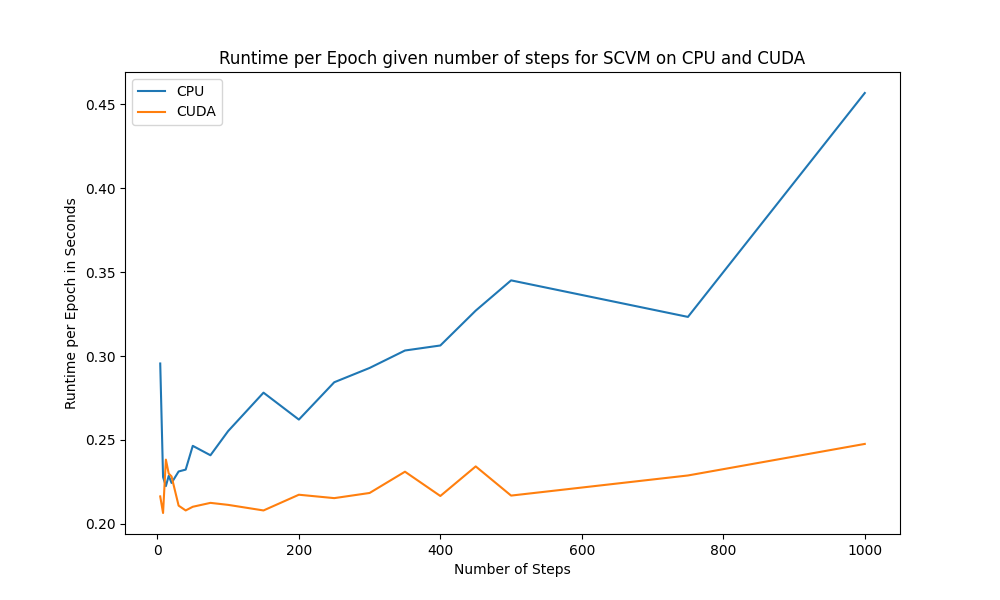
\includegraphics[width=\textwidth]{0_images/steps_runtime2.png}
    \caption{Run time of the SCVM relative to the number of steps}
    \label{fig:NumStepsRuntimes}
\end{figure}
\textbf{Number of Interactions}
\\
The third and final scalability test is carried out with the goal of evaluating the impact on run time the dataset size has.
For this test, the data is generated based on the $\beta$-value, taken from the range:
\begin{equation}
    \beta = [5.0, 5.25, 5.5, 5.75, 6.0, 6.25, 6.5, 6.75, 7.0, 7.25, 7.5, 7.75, 8.0, 8.25, 8.5, 8.75, 9.0]
\end{equation}
The number of interactions generated from these beta values are as follows:
\begin{equation}
    n = 
\end{equation}

The dataset is generated using $N = 4$ nodes, and SCVM has to fit four velocity vectors to each node, ie. four steps.
Once again, for each dataset size, the mean run time per epoch over five runs are recorded for both the CPU and CUDA.

Figure \ref{fig:NumInteractionsRuntimes} below shows the run times per epoch given the number of steps the SCVM has to fit, using the CPU (in blue) and CUDA (in orange).


\begin{figure}[H]
    \centering
    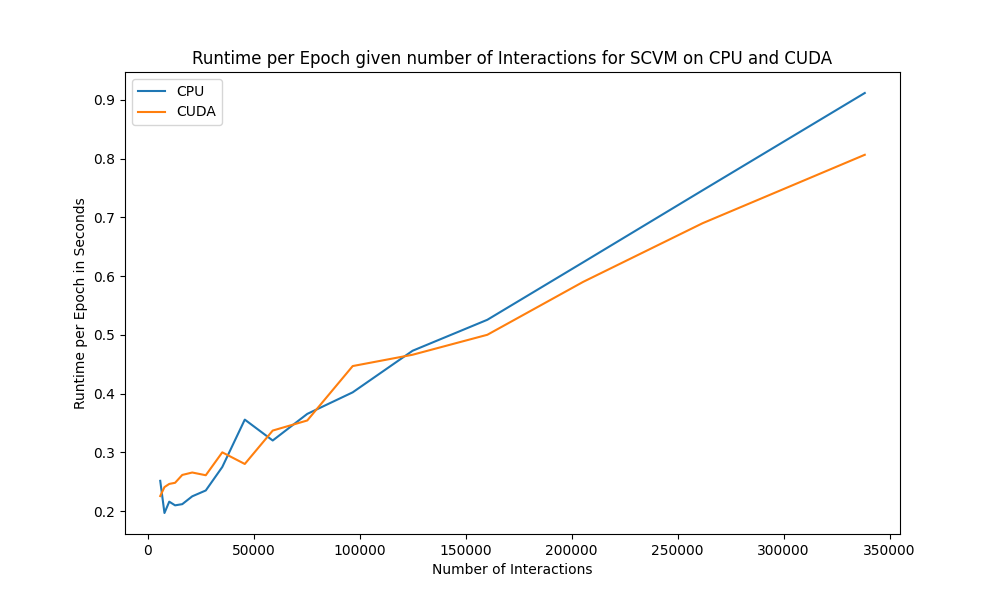
\includegraphics[width=\textwidth]{0_images/numinteractions_runtime2.png}
    \caption{Run time of the SCVM relative to the number of interactions}
    \label{fig:NumInteractionsRuntimes}
\end{figure}
\clearpage
\subsection{Third Research Question}
\label{sec:ResearchQuestion3}
The third research question of this project states:
\\
"How can the model be visualized to enforce explainability?"



\subsubsection{Lyon Primary School dataset}
\label{sec:ResearchQuestion3:LyonDataset}

Real dataset 3, see section \ref{sec:Data:RealData:RealDataset3}, is utilized here.
\\\\
\textbf{Animation check without position correction and discussion.}


\textbf{Animation check with position correction and discussion.}


\textbf{Animation check with regularization and discussion.}




\clearpage

\section{Discussion}
\label{sec:Discussion}
This section first of all discusses the overarching takeaways that the results have posed.
It then discusses the future work that should be done in order to expand the capabilities of the proposed model.
Finally, it dives into the future prospects of use that this technology poses.
\subsection{Discussion of Results}
\label{sec:Discussion:Results}


\subsubsection{Bias Term $\beta$}
\label{sec:Discussion:Results:BiasTerm}
The use of a dataset-wide bias term is possibly insufficient in terms of correctly representing the different nodes of the TDGN the model is trying to model. 
This fact is of course not true for the synthetic dataset results, as the data of these sets are all generated from a single beta value, but for the real datasets it might very well be the case.

In a given network, a very plausible scenario may be that some entities are less active than others, and the model then fits a beta value that reflects greater background intensity than these entities entail.
In order to compensate for this, the model will place these less active entities further away from the more active entities, neglecting the proportions of each individual node's overall interaction intensity.

A fitting expansion of the model would hence be node-specific bias terms, with which every node is attributed it's own beta value, and as such can be spatially modelled in latent space while accounting for the node's overall interaction intensity. 
\\\\
For the proposed SCVM, the fact that the different steps are governed by the same bias term may also be a limitation. 
The mean intensities for each step may vary a lot, just as with the individual nodes.
Hence, another expansion in relation to the bias term would be to have step-specific bias terms, each governing the background intensity of the given step.
\\\\
The combination of the node-specific bias term and the step-specific would then be the node-step-specific bias term, learning a beta parameter for each node for each step.


\subsubsection{Alternative Training Setup}
\label{sec:Discussion:Results:AlternativeTrainingSetups}
For this project, the training was carried out using the Pytorch Ignite framework, and during all training epochs, the parameters $\beta$, $z0$ and $v0$ were all optimized at the same time.
This training setup was deemed appropriate for the SCVM, as it was able to converge well given a training length of 5000 epochs.

The length of the training was made possible by the speedup in computation, a result of improving scalability through vectorization, as well as the fact that the datasets used used in this project were of a certain maximum size.
For \textit{even} larger dynamic networks, perhaps with several thousand nodes and several millions of interactions, the training of the SCVM would take days at least, which in many cases poses as unfeasible. 

In order to enable training of larger dynamic networks in a feasible time frame, convergence of model parameters should ideally happen on the basis of relatively fewer epochs.
One way to potentially realize this solution would be to run a sequential training setup, in which some parameters are initialized and learned before others.
For the SCVM, this would mean initializing only the position parameter $z0$ first, and for the first third of the training only seek to optimize the model by changing the initial positions.
Then, the model would initialize the velocities for all nodes, and for the middle third of training fit only the positions and velocities. 
Lastly it would seek to optimize the model based on all three parameters.




\subsubsection{Computation Times and Memory Limitations}
\label{sec:Discussion:Results:MemoryLimitations}
In the results for research question 2, see section \ref{sec:ResearchQuestion2}, it was shown how the proposed vectorized setup improved scalability to such extend that it reduced the run time for training on synthetic dataset 1 by around a factor 32.

The subsequent section, regarding computational speed, gave a more detailed overview of the running times of the vectorized setup, in relation to number of nodes, steps and interactions.
The results showed that both when increasing the number of nodes in the dataset, as well as the number of steps the SCVM had to fit, the run times where similar for low numbers, but increased seemingly exponentially when running the training on the CPU, and relatively linearly when training using CUDA.
The explanation for these results seem rather straight forward; the vectorized setup enables parallization, enabling the computations to be run in parallel on multiple cores, of which the GPU has in abundance compared to the CPU. 
Specifically, the CPU, an Intel Core i7-9750H, used for generating these results has 6 cores (with multi threading this number is actually 12) while the GPU, an NVIDA GeForce GTX 1650, has 896 CUDA cores.
In theory, this means 896 calculations can happen simultaneously compared to 12.

The size of the dataset, ie. number of interactions, resulted in the same run times for both the CPU and CUDA.
This 
\\\\
A problem which was met when running larger dynamic networks, of $N = 100$ nodes and more, was the memory requirement.
With an increased number on unique nodes, the amount of memory needed to be allocated expands fast due to the tensor having dimensions that are $N \cdot Num_Steps \cdot n$
\\\\
Improvement to be made for the vectorized setup consist first and foremost in handling the memory requirement. 
The code underlying the proposed model is not optimed in terms of reducing memory requirement, this could potentially be done, but as of now we are not familiar with the 'how'.







\subsection{Future Work and Improvements}
\label{sec:Discussion:FutureWork}
The work of this project takes a big step towards utilizing the latent space modelling approach as a detailed, scalable means of modelling dynamic networks in an explainable way.
In regards to the implemented model, the discussion points regarding the results discuss potential improvements that could be made to the already implemented components that make up the SCVM and visualisation. 
In order to fully realize the potential of the modelling approach though, some further, new components could advantageously be added on top of the work presented in this project.


\subsubsection{Memory Limitations}
\label{sec:Discussion:FutureWork:MemoryLimitations}
A problem which was met when running larger dynamic networks, of $N = 100$ nodes and more, was the memory allocation requirement.
With an increased number of unique nodes and an increased number of steps, the amount of memory needed to be allocated expands fast due to the tensor having dimensions of $N \times 2 \times S$, ie. number of nodes times number of dimensions (2) times number of steps. 
Further, the number of unique nodes is an even greater limiting factor, since the node pairwise computations are performed on $S$ $N \times N$ matrices, hence growing exponentially with $N$.
An improvement to be made for the vectorized setup consist first and foremost in handling this memory requirement. 
The code underlying the proposed model is not particularly optimized in terms of reducing memory requirements, as the focus has mainly been on optimizing the scalability in regards to run time. 
\\
One way the memory requirements could potentially be reduced though, would be by splitting up the computation of node interaction intensities through batching of the nodes. 
This is in theory easily done, as the computations of each node batch intensity can be computed and summed, thereby keeping an upper limit on how many nodes are included in each computation. 
\\
Another approach could be to not directly do node-wise batching, but instead (or also) use multiple GPUs. 
This approach was considered during the project, but due to large queue times on the DTU HPC servers when requesting multiple GPUs, did not come to fruition. 
This should however quite easily be done by using the Pytorch DataParallel \cite{DataParallelDocumentation} class and specifying multiple device IDs. 
\\
Yet another way of improving memory utilization would be to check the model consistently to ensure objects sent to the GPU device are detached optimally when no longer used.
Further, checking and converting data types that can be reduced in size, e.g. float64 to float32, could be explored.
Also, exploring the possibility of using sparse data representations \cite{Torch.sparseDocumentation} for large tensors would be interesting.


\subsubsection{Bias Term $\beta$}
\label{sec:Discussion:Results:BiasTerm}
The use of a dataset-wide bias term is possibly insufficient in terms of correctly representing the different nodes of the dynamic network. 
This fact is of course not true for the synthetic dataset results, as the data of these sets are all generated from a single beta value, but for the real datasets it might very well be the case.
In a given network, a very plausible scenario may be that some entities are less active than others, and with the current setup, the SCVM fits a $\beta$ value that reflects greater background intensity than these entities entail.
In order to compensate for this difference in average intensity, the SCVM will place these less active entities further away from the more active entities, hence neglecting the proportions of each individual node's average interaction intensity.
A fitting expansion of the model would be the implementation of node-specific bias terms, with which every node is attributed its own beta value, and as such can be spatially modelled in latent space while accounting for the node's average interaction intensity. 
\\
For the proposed SCVM, the fact that the different steps are governed by the same bias term may also be a limitation. 
The average intensities for each step may vary a lot, just as with the individual nodes.
Hence, another expansion in relation to the bias term would be to have step-specific bias terms, each governing the background intensity of the given step.
\\
Finally a combination of the node-specific bias term and the step-specific would then be the node-step-specific bias term, learning a beta parameter for each node for each step.


\subsubsection{Alternative Training Setup}
\label{sec:Discussion:Results:AlternativeTrainingSetups}
For this project, the training was carried out using the Pytorch Ignite framework, and during all training epochs, the parameters $\beta$, $z0$ and $v0$ were all optimized at the same time.
This training setup was deemed appropriate for the SCVM, as it was able to converge well given a training length of 5000 epochs, which could be completed in a feasible time frame.
The length of the training was made possible by the speedup in computation, a result of improving scalability through vectorization, as well as the fact that the datasets used in this project were of a certain size.
\\
When training on the Lyon dataset, which has 237 nodes and 3.5 million interactions, fitting 249 steps, the training time was around 14 hours when running on an NVIDIA GTX 1650 GPU.
For \textit{even} larger dynamic networks, perhaps with several thousand nodes and several millions of interactions, the training of the SCVM will likely take days at least, which in many cases poses as infeasible. 
In order to enable training of such large dynamic networks in a manageable time frame, convergence of model parameters should ideally happen on the basis of relatively fewer epochs.
One way to potentially realize this would be to run a sequential training setup, in which some parameters are initialized and learned before others.
For the SCVM, this could mean initializing only the position parameter $\textbf{Z}$ first, and for the first proportion of the training, say a third, only seek to optimize the model by changing the initial positions.
Then, the model would initialize the velocities for all nodes $\textbf{V}$, and for the middle third of training fit only the positions and velocities. 
Lastly, the SCVM it would train the model while also fitting the $\beta$ parameter.
\\
Another solution, as presented for solving the memory limitations, would be to use multiple GPUs either through Pytorch or scale up to multiple clusters through other frameworks like Apache Spark\cite{ApacheAnalytics}.
Distributing the computations would enable a greater use of parallelization, likely improving run times by a significant amount.

\subsubsection{Optimizing Visualizations}
For creating the animations in this project, a simple dataframe of the learned parameters together with an animated plotly \cite{PlotlyPlotly} scatter plot is used. 
However, the animation process could be made far more scalable by using other available frameworks for graph creation and visualization, and allow for higher time-resolution animations to be created. 
One such framework is Graphviz \cite{Graphviz}, which is optimized specifically for graph visualizations, and could advantageously be used in future work. 
Using Graphviz should first of all make the visualizations scale to even larger amounts of nodes higher time-resolutions. 
Also, edges are an integrated part of Graphviz, and the framework would therefore allow for easy visualizations of edges between nodes, when they interact according to the input data. As mentioned in the discussion about the results of research question 3, this could increase the interpretability of the visualizations even further. 
\subsection{Real World Applications}
\label{sec:Discussion:UseCases}
The proposed SCVM represents the possibility of modelling larger dynamical networks in latent space using Newtonian dynamics.
While not many dynamic networks are based in Newtonian dynamic, the stepwise approach enables for the modelling of non-Newtonian dynamic networks with greater detail than previous work, while retaining the ease of explainability that Newtonian dynamics in latent space provides.

In this regard, the SCVM 


\subsubsection{Hospitals}
\label{sec:Discussion:UseCases:Hospitals}
Hospitals logging.



\subsubsection{Marketing}
\label{sec:Discussion:UseCases:Marketing}
Edge prediction: Determine nodes that are most likely to interact in the future, but aren't currently.

\clearpage


\section{Conclusion}

During the investigations conducted in this project, the posed research questions were answered and a number of insights were found:
\\\\
First of all, the results regarding research question 1 showed that the proposed SCVM had good modelling performance when comparing modelled intensity rates to ground truth models, and naturally outshone previous work when modelling multi-step, synthetically generated dynamic network data.
The tests of dyad removal and interaction removal revealed less striking performance, which might be resulting from the nature of the synthesized datasets. 
To clearly determine the reason for the low performance, more tests have to be conducted.
Nonetheless, the project concludes that the proposed SCVM, specifically through the introduction of stepwise computation, is able to model the interactions of dynamic networks well, with more detail than previous work.
\\\\
The project sought to implement the proposed model in a scalable manner, and the results presented for research question 2 proved that this was achieved with success.
The training times for the vectorized setup was found to be 32 times faster when fitting four nodes with one step, using the CPU, compared to the baseline non-vectorized setup.
In relation to number of nodes, steps and dataset size, the training run times for the proposed training setup were evaluated when running on either the CPU or the GPU using CUDA.
While the run times grew similarly for larger dataset sizes, increasing either number of nodes or steps showed the significant improvements parallelization provides, as it enables full use of the CUDA system. 
In this regard, the proposed model is definitely scalable in terms of computation.
The project discussed limitations to scalability which arise with memory allocation requirements, but found that several solutions to this limitations could be implemented without changing the SCVM training setup in any significant way.
As such, the project concludes that the SCVM was in fact implemented in a scalable manner, to great extend making the modelling of larger networks feasible.
\\\\
With the proposed SCVM, a goal was to create visualizations that are explainable and interpretable for an observer, as to understand the dynamics of a given network.
The results showed that visualizations of datasets based on real dynamic networks could be made so that the network could be inspected at any given time during its duration.
The results regarding explainability evaluated the impact of applying position, drift and rotation correction as well as regularizing the model.
It was found that position and drift correction immediately made for a more interpretable visualization, while correcting rotation was deemed to be an enhancement which mostly improves comparability between different networks.
While regularization was found to slow the movements of nodes down, it was not found to inherently improve the overall explainability of the modelled dynamic networks used in this project.
The project concludes, that while the visualizations produced by the SCVM could advantageously be expanded as to deliver more information in order to improve explainability, animating entities in a dynamic network as nodes with stepwise constant velocity dynamics allowed for an intuitive interpretation of how the nodes relate over time. 
\\\\
Some possibilities of future expansions to the proposed SCVM were discussed, including the introduction of node-specific and step-specific bias terms, as to possibly model a dynamic network with greater detail.
\\\\
Lastly, the project briefly discussed some possible real life use cases the proposed model could be utilized in, one of these being work flow modelling and optimization at hospitals. 
The project further argued that the SCVM-produced embedding of a given dynamic network could potentially be utilized for some machine learning task. 


\clearpage

%\bibliographystyle{unsrt}
%\bibliography{references}
\printbibliography
\clearpage

\section*{Appendix}
\appendix
%Use appendix by inputting seperate files.
%DO NOT WRITE APPENDIX TEXT DIRECTLY HERE IT WILL BE TOO LONG

%test file to show how to add files to the appendix
%\input{appendix/sanity_check_speakers}



\end{document}
